% Activate the following line by filling in the right side. If for example the name of the root file is Main.tex, write
% "...root = Main.tex" if the chapter file is in the same directory, and "...root = ../Main.tex" if the chapter is in a subdirectory.
 
% !TEX root = ../thesis.tex 

\chapter{Literature review}
\label{lit_review_chapter}

\section{Anatomy and physiology of the brain}

The brain is comprised of left and right symmetric hemispheres. The narrow void between the outer surface of the brain and the cranium within which it is contained is taken up by cerebrospinal fluid (CSF). The voids found at the centre of each hemisphere, named lateral ventricles, also contain CSF. The outer surface of each hemisphere is comprised of a thin and highly folded sheet of grey matter (GM) tissue, named the cerebral cortex. The most exterior and most interior portions of the folds on the cortical surface are named gyri and sulci respectively. The majority of the volume interior to the cortex (the subcortex) is composed of white matter (WM) tissue. Finally, deep within the subcortex there exist a number of structures that are also comprised of GM; these may variously be referred to as deep or subcortical GM structures. One such example is the hippocampus. An illustrative overview of these tissues and structures is given in figure \ref{anatomy}. 

\begin{figure}
\centering
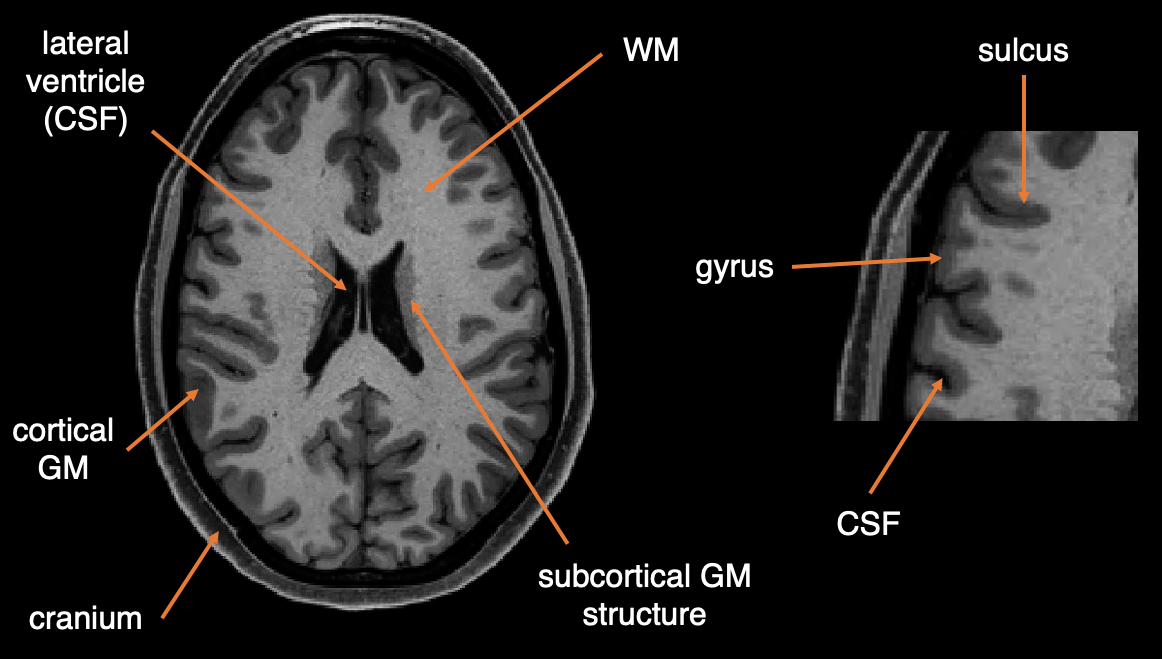
\includegraphics[width = \textwidth]{anatomy.png}
\caption{Left: High-level anatomy of the brain, showing the location of GM (cortical and subcortical), WM and CSF. Right: detail of the cortex, showing sulci and gyri.}
\label{anatomy}
\end{figure}

In a broad manner of speaking, the cortex performs many important tasks of cognition and accordingly it has been the focus of much research in neuroanatomy and brain function. To this end, researchers have identified numerous small and functionally distinct areas of cortex, for example the visual and auditory cortex, which process and respond to visual and aural stimuli respectively. Such a segmentation by function is commonly referred to as a \textit{parcellation} and an example is the Human Connectome Project's (HCP) multi-modal parcellation \cite{Glasser2016}, illustrated in figure \ref{fig_hcp_mmp}. In consequence of its many functions, the cortex is very physiologically active and has a high metabolic demand for oxygen and glucose, delivered via blood. Each of these metabolic demands can be used as a basis for physiological imaging, namely: 

\begin{itemize}

\item blood-oxygenation level dependent magnetic resonance imaging (BOLD MRI) is sensitive to the changes in blood oxygenation that accompany neuronal activation \cite{Jenkinson2017a}; 

\item fluorodeoxyglucose positron-emission tomography (FDG PET) is sensitive to changes in glucose metabolism \cite{Bohnen2013}; 

\item and arterial spin labelling MRI (ASL MRI) is sensitive to changes in blood delivery, a process called \textit{perfusion} \cite{Alsop2015}.  

\end{itemize}
 
\begin{figure}
\centering
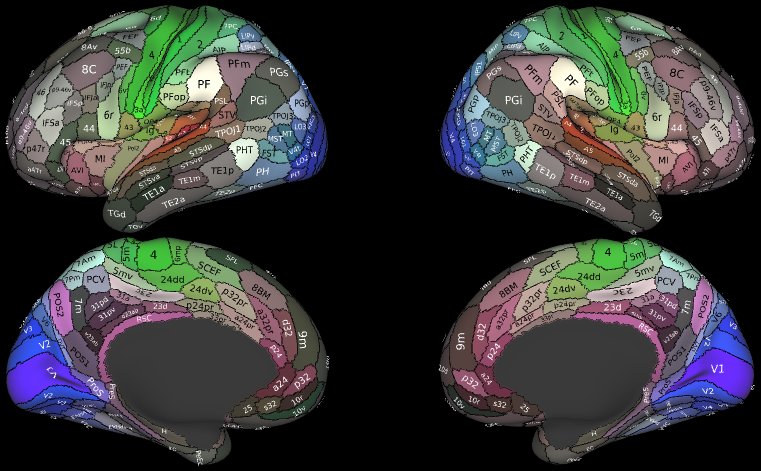
\includegraphics[width = 0.9\textwidth]{hcp_mmp.png}
\caption{The HCP-MMP parcellation of the left and right cortical hemispheres, coloured according to high-level function. For example, blue regions are associated with visual tasks. Reproduced with permission from \cite{hcp_mmp}.}
\label{fig_hcp_mmp}
\end{figure}

The function of WM in the subcortex may simplistically be described as providing connections between different parts of the cortex, and in consequence it is often discussed in context of the \textit{connectome}, a general term that describes the architecture of connections that form the basis of network-based models of cognition \cite{Sporns2005}. Though it is less physiologically active (being perfused at a lower rate than the cortex), it is by no means a passive tissue and is the focus of increasing amounts of research, particularly concerning neurodegenerative disease. For example, degradation of the myelin sheaths that surround axons plays a key role in multiple sclerosis \cite{Shafee2015}. As a result of its reduced levels of activity compared to the cortex, it can be challenging to perform physiological imaging in WM (the signal to noise ratio is inherently lower for some modalities). 

\section{Physiological imaging via arterial spin labelling}

Arterial spin labelling is a physiological imaging modality that uses magnetic resonance to produce signal. In common with other physiological imaging modalities (notably, PET), signal is acquired in a volumetric manner. The imaging region is divided into a regular grid of discrete subunits (voxels) within which signal is aggregated. The resultant data is stored as a three-dimensional matrix (with time acting as a fourth dimension where necessary) that matches the discretisation of the imaging region.
 
\subsection{The magnetic resonance signal}

Magnetic resonance imaging (MRI) is a non-invasive volumetric imaging technique that uses the magnetic properties of hydrogen nuclei to generate signal \cite{bushberg2011}. In the presence of an external magnetic field, a population of hydrogen nuclei, referred to as \textit{spins}, will align their spin axis with that of the field and precess in steady-state with a well-defined frequency. The principle of MRI is to disturb this steady-state with radio-frequency (RF) excitation pulses that match the resonant frequency of spins and measure the dynamics of how steady-state is restored. The strength of the resonance signal is determined by the density of spins present in the imaging region and two physical decay constants. Different forms of MRI are distinguished by the sequence of RF pulses that they use to excite spins and subsequently acquire signal. 

%\subsection{Image acquisition} 

%Starting from a condition of steady-state, spins are aligned with the external magnetic field along the longitudinal axis (corresponding to the scanner bore and the inferior-superior axis of the patient). An RF excitation pulse instantaneously `tips' them into a transverse plane, from which they will re-align themselves over time with the longitudinal axis. Whilst the spins are returning to steady state, they emit an RF signal in the transverse plane that can be recorded by a set of readout coils and ultimately be converted into an image. The time between successive RF excitations is known as repetition time (TR). Signal acquisition is performed a short time after an RF excitation pulse; the period is known as the echo time (TE). In order to improve image quality, many repetitions of the excite/acquire process are performed. TE tends to be on the order of tens of milliseconds, whereas TR is usually a few seconds.   

%A spatial encoding strategy is used to localise the MR signal with respect to the position of the imaging region from which it originated. As a necessary step in this process, the imaging region is discretised into a regular grid of volume element, referred to as voxels. The resultant image will contain the summation of all signal contributions within the region of space corresponding to each voxel. For structural MRI, voxel sizes are usually around 1mm isotropic. 

%Signal acquisition is performed in the frequency-phase domain and a spatial encoding strategy is thus required to map positions within the imaging region to positions within the frequency-phase domain. Though there are many strategies for doing so, a common and simple approach is to use a series of 2D `slice' acquisitions which are then stacked into a single 3D volume. Under this approach, the slices are conventionally acquired along the increasing z-axis, from inferior to superior as referenced to the patient. Within an individual slice, frequency gradients and phase offsets are used to encode positions on the x-y plane. A Fourier transform is then applied to the frequency-phase data to reconstruct individual image slices. MR images are volumetric in nature and are comprised of many individual `voxels' (volume pixels). Voxels are a property of the spatial encoding strategy that was used to acquire the image and represent the discretisation of real space over which the MR signal was sampled. For typical anatomical MR scans, the voxel size is on the order of 1mm isotropic. 
 
\subsection{Control of contrast}

MRI allows image contrast to be controlled according to the magnetic properties of tissue. The resonance signal is subject to two forms of exponential decay, named T1 and T2 after the time constants that govern them. T1, or longitudinal, decay is the process by which a population of spins return to their equilibrium state following an excitation RF pulse. T1 is usually on the order of 1 - 2s for human tissue \cite{Alsop2015}. T2, or transverse, decay is the process by which a population of resonating nuclei de-phase relative to each other whilst out of alignment with the external field, thereby reducing the strength of their overall signal. T2 is on the order of 100ms for human tissue \cite{Buxton2009}. Strictly speaking, transverse decay is governed by a more complex constant called T2*, however commonly-used refocussing strategies remove the effect of this constant and it is therefore left out of this overview \cite{bushberg2011}. 

Two parameters of an MRI acquisition, referred to as the echo time (TE) and repetition time (TR), can be varied to maximise contrast as a function of tissue T2 or T1 respectively. For example, if TR is set to be many periods of T1, e.g. 7s, then all tissues are said to `fully relax' in the period between successive excitations and there will be little contrast arising from T1 differences. Conversely, for a short TR of 2s there will be some tissues that relax more than others, leading to greater image contrast. Control over contrast in this manner is referred to as \textit{weighting} the image; examples of T1-weighted and T2-weighted structural MRI scans are given in figure \ref{t1t2_image}. 

%\begin{table}
%\centering
%\def\arraystretch{1.5}
%\begin{tabular}{p{1cm} | p{6cm} | p{6cm}}
%& Short TE & Long TE \\
%\hline
%Short TR & T1-weighted: little de-phasing (T2) but tissues cannot fully relax longitudinally (T1)   & Mixed T1 and T2 image \\
%\hline
%Long TR & Proton density image: little de-phasing (T2) and full relaxation (T1) & T2-weighted: significant dephasing (T2) and full relaxation (T1)
%\end{tabular}
%\caption{TE and TR combinations to vary image contrast in MRI}
%\label {tableImageWeighting}
%\end{table}

\begin{figure}[h]
\centering
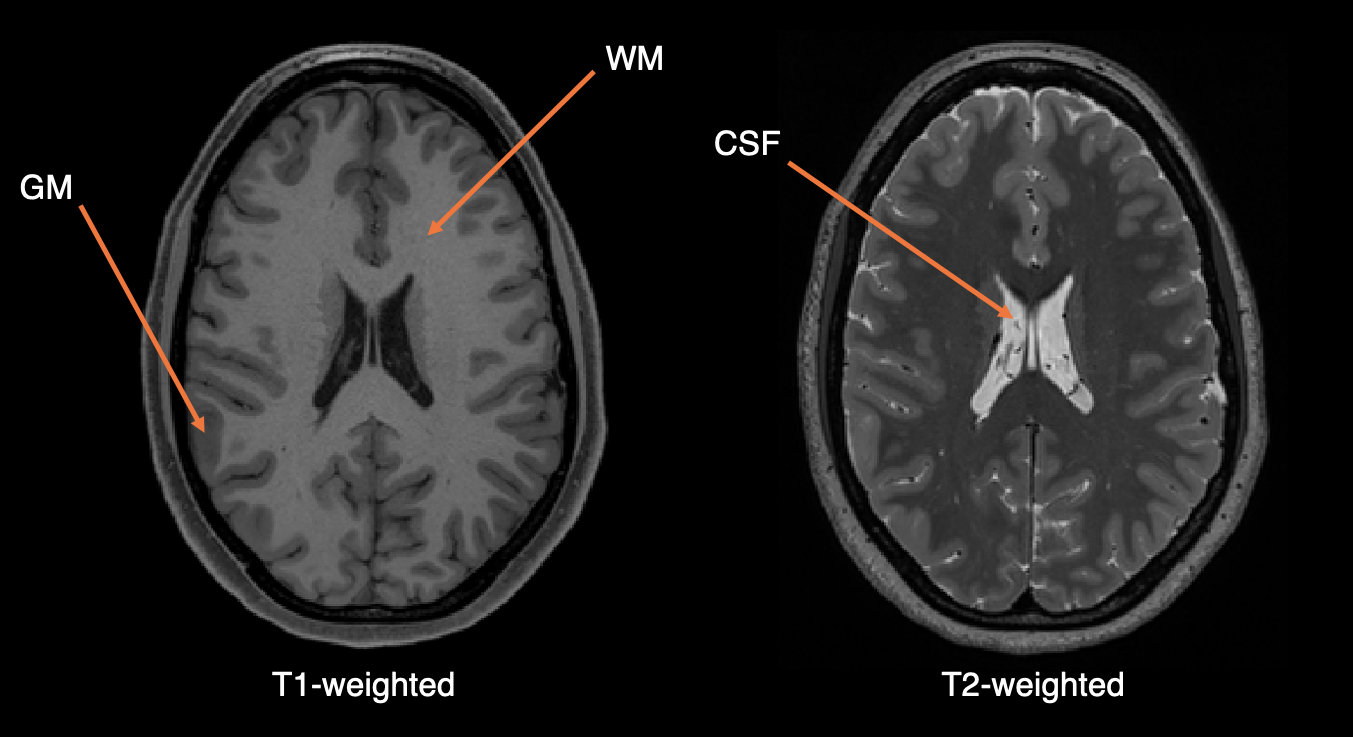
\includegraphics[width = \textwidth]{t1t2.png}
\caption{T1-weighted and T2-weighted structural MR images for subject 103818 of the HCP. Tissue intensities are broadly inverted between the two weightings (for example, CSF is dark on the T1w and light on the T2w), demonstrating how image contrast can be varied according to the T1 and T2 properties of tissue.}
\label{t1t2_image}
\end{figure}


\subsection{The arterial spin labelling signal}

Arterial spin labelling (ASL) is a non-invasive MRI technique that uses arterial blood-water as an endogenous contrast agent to measure the dynamics of perfusion \cite{Alsop2015}. Using magnetic fields, it is possible to magnetically `label' blood, follow its subsequent progression through the vasculature and exchange into tissue (the process of perfusion). Two parameters are of particular interest: cerebral blood flow (CBF) is the rate of blood delivery per unit weight of tissue, and arterial transit time (ATT) is the time taken for blood to traverse the vasculature.  

An ASL acquisition entails gathering many \textit{label} and \textit{control} image pairs \cite{asl_primer}. Using ASL applied to the brain as an example, a labelling region is defined across the neck perpendicular to the carotid arteries that supply blood to the brain. Prior to each label image acquisition, RF energy is applied within the region to invert the magnetic moment of spins that are present. The labelling itself may be instantaneous (referred to as pulsed ASL, pASL, in which case the region is a few centimetres thick) or maintained for a set length of time (referred to as continuous or pseudo-continuous ASL, pcASL, in which case the region is a plane of negligible thickness). The two labelling strategies are illustrated in figure \ref{label_regions}. The total quantity of blood that is inverted is referred to as the \textit{bolus} of label and is typically measured by duration, for example, a bolus of duration 1s. For pASL, the bolus duration is necessarily an approximate quantity as an entire spatial region is inverted instantaneously in time, though there are strategies that can be used to give a better-defined bolus duration (for example, QUIPSS II \cite{asl_primer}). 

\begin{figure}[h]
\centering
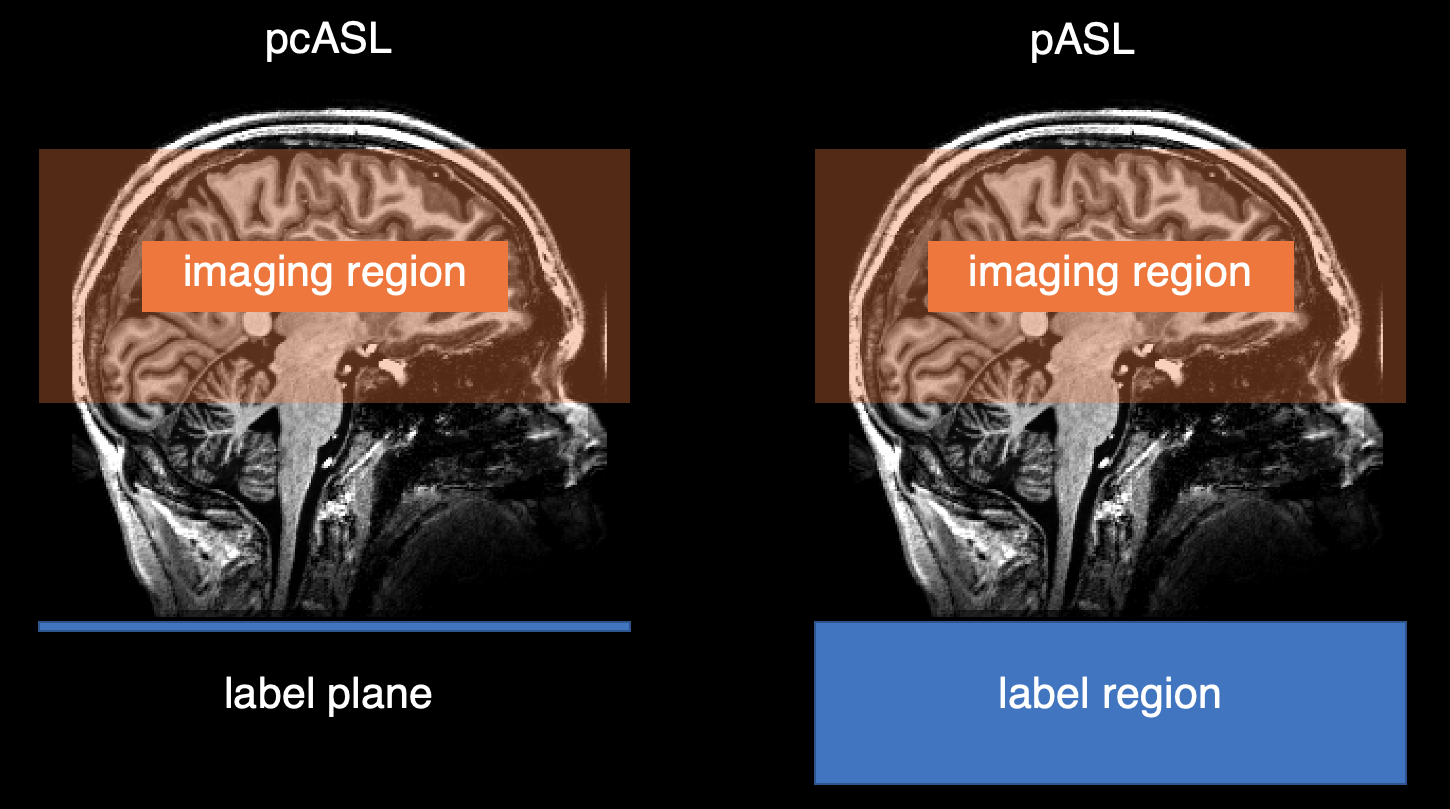
\includegraphics[width = \textwidth]{pcasl_pasl_regions.png}
\caption{Imaging and label regions for pcASL and pASL. For pcASL, the labelling is performed across a plane for a set time, for pASL it is performed instantaneously within a region.}
\label{label_regions}
\end{figure}

After labelling, a further period of time (known as the inversion time, TI, for pASL, or post label delay, PLD, for pcASL) elapses before image readout is performed. The TI/PLD allows the label bolus to traverse the arterial network and be delivered to the capillary bed of cerebral tissue (the length of time this requires is the arterial transit time, ATT). The entire process of label creation to readout leads yields a single label image. A control image is acquired in the same manner, except no RF inversion is applied and no label is created. The two images together comprise a label-control pair, the smallest unit of data required for the measurement of perfusion via ASL. 

Perfusion leads to the delivery of label, i.e. magnetically inverted spins, to the capillary bed, after which it exchanges into cerebral tissue. In the ideal case, when a label and control image are subtracted from each other, any cerebral tissue that was not perfused will have the same magnetisation on both images and produce zero difference signal. By contrast, tissue that has been perfused will have a lower magnetisation on the label image and hence produce a non-zero difference. The result of a label-control subtraction is referred to as a perfusion-weighted image and is the simplest possible indicator of perfusion available from ASL data, though it does not give quantitative estimates of CBF or ATT directly. 

The subtraction of a label-control pair yields a very weak signal. The difference image typically has around 1\% of the signal magnitude of the control image itself, and as such ASL suffers from intrinsically poor signal-to-noise-ratio (SNR) \cite{Li2018}. Based on the assumption that noise within an ASL acquisition follows a zero-mean Gaussian distribution (additive `white' noise) a number of strategies may be used to overcome this. Firstly, multiple label-control pairs can be acquired, across which the effects of noise should average out (taking multiple measurements of a noisy signal should yield the underlying true value, as is illustrated in figure \ref{single_multi_noisy}). Secondly, creating larger label boluses directly increases the magnitude of the difference signal. Finally, increasing the voxel size of the acquisition causes the difference signal to be sampled over a larger volume of space per voxel, which again causes noise to average out. It is for this latter reason that ASL data tends to have much larger voxel sizes than structural MRI (3-4mm vs. 1mm). Each of these strategies imposes a penalty: the first two directly increase the total duration of the acquisition, whereas the latter reduces the ability to resolve spatial details within the image. 


\subsection{The kinetic model for ASL} 
\label{asl_kinetic_section}

With appropriate processing, label-control difference images may be used to give absolute quantification of CBF and ATT \cite{asl_primer}. This is achieved by fitting a kinetic model of perfusion to the data in order to estimate the physiological parameters of interest. This model (hereafter referred to as the general model) is developed by considering the delivery of label to, and removal from, each voxel of the imaging region. The former process is represented by the arterial input function (AIF) and the latter by the residue function. As is the case for other tracer imaging techniques, the general model is formed by the convolution of the AIF with the residue function \cite{Buxton1998}. Conceptually, this is equivalent to splitting the label bolus into infinitely many discrete time intervals that are delivered independently, letting each of them decay after arrival \textit{on their own time scale}, and then summing their individual contributions at all moments in time. 

\subsubsection{Arterial input function}

In the ideal case, the label bolus is perfectly rectangular in time and space: it arrives uniformly, continues to do so for a length of time equal to the bolus duration $\tau$, and then ceases. During the time period between label creation and arrival in the imaging region (the ATT, denoted $t_A$), the label bolus will decay due to T1 effects, with the rate fixed by the T1 value of blood. The AIF is therefore a time-shifted and decayed copy of the original label profile. For pcASL, each part of the bolus takes the same time to travel from the label plane to the imaging region (fixed by the ATT), so each part of the bolus experiences the same decay and the profile is rectangular. For pASL, in which all of the bolus is created \textit{at the same time}, the leading edge reaches the imaging region before the trailing edge and therefore experiences less decay. The profile is therefore a windowed exponential decay curve, with the length of the window equal to the bolus duration. These are both illustrated in figure \ref{aif_profiles} and their mathematical forms are given in equation \ref{aif_functions}. The magnetisation of blood within the labelling region is denoted by $M_{0a}$. It is also possible to account for dispersion effects in the AIF (in reality, flow is non-uniform through the vasculature), though this effect is generally neglected \cite{asl_primer}. 

\begin{equation}
  a(t) =
  \begin{cases}
    0 & \text{for } t < t_{A} \\
    2M_{0a}e^{-(t-t_{A})/T_{1b}} & \text{(pASL) for } t_{A} \leq t < \tau + t_{A} \\
    2M_{0a}e^{-t_{A}/T_{1b}} & \text{(pcASL) } \\
    0 & \text{for } \tau + t_{A} \leq t \\
  \end{cases}
  \label{aif_functions}
\end{equation}


\begin{figure}[H]
\centering
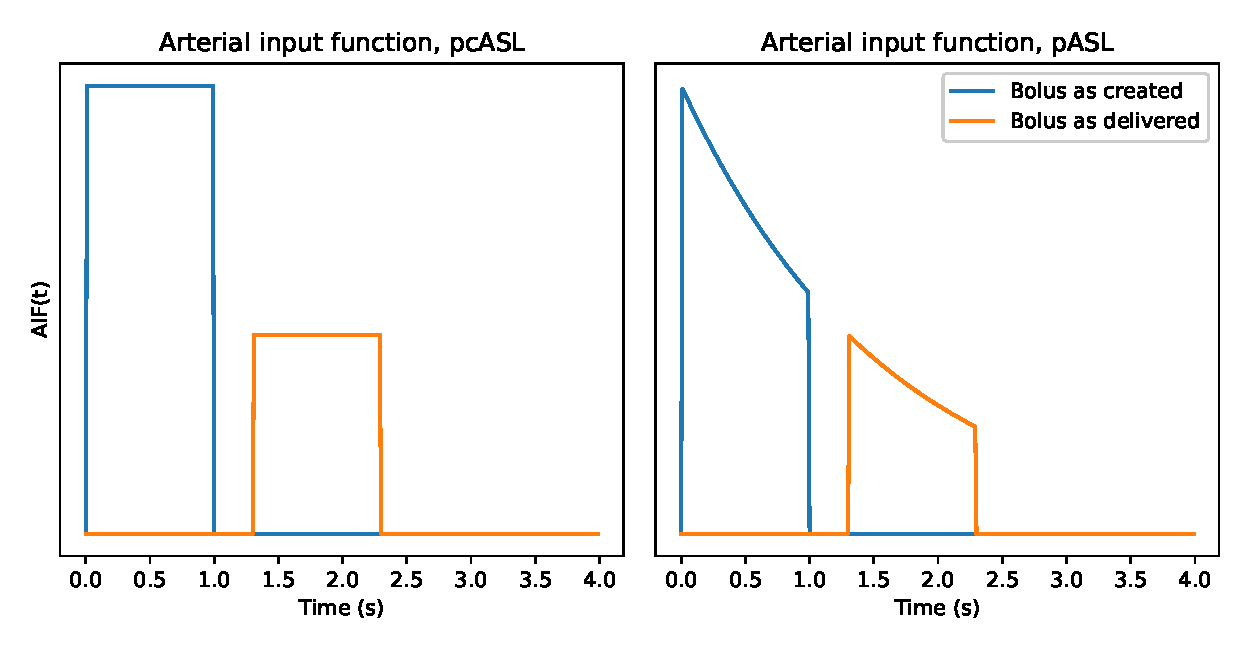
\includegraphics[width = 0.9\textwidth]{aif_profiles.eps}
\caption{AIF profiles for pcASL (left) and pASL (right) with 1s bolus duration and 1.3s ATT. The effect of T1 decay between label creation and delivery is shown; the rate of decay is fixed by the reference T1-blood value of 1.6s.}
\label{aif_profiles}
\end{figure}

\subsubsection{Residue function}

Upon arrival in the imaging region, the label bolus is removed by two processes. Firstly, it may leave by passing through the venous side of the capillary bed, a process that depends on the CBF $f$ of the voxel itself and also the partition coefficient $\lambda$, the relative concentration of water between the vascular space and tissue. Secondly, the label bolus will experience T1 decay, although the rate of this will now be fixed by the T1 value of the \textit{surrounding tissue}, not the T1 value of blood itself. This follows from the assumption that the exchange of label into tissue upon arrival in the voxel is fast; the voxel is said to be `well-mixed' \cite{Buxton1998}. The residue function is illustrated in figure \ref{residue_fig} and the mathematical form given in equation \ref{residue_eqn}. 

\begin{equation}
r(t) = e^{-tf/\lambda} \cdot e^{-t/T_{1}}
\label{residue_eqn}
\end{equation}

\begin{figure}[H]
\centering
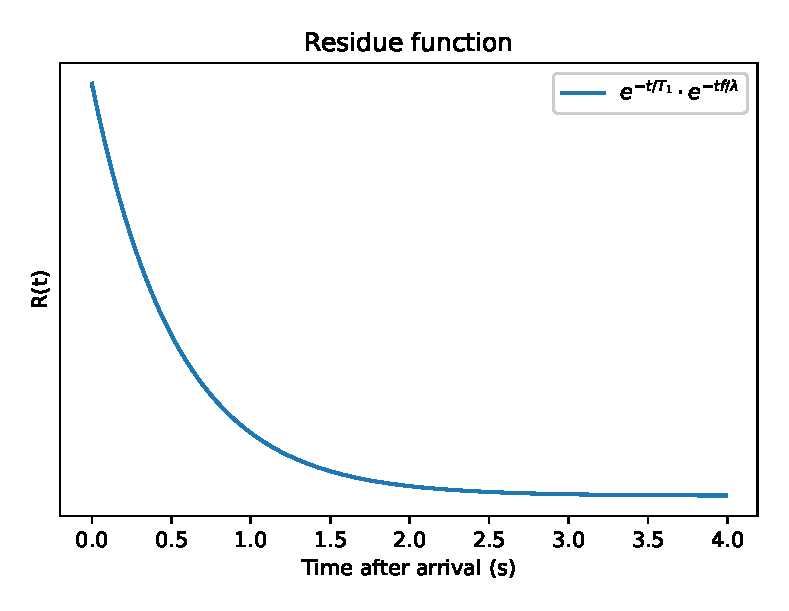
\includegraphics[width = 0.6\textwidth]{residue.eps}
\caption{Residue function for delivered label. The rate of decay is fixed by the T1 value of surrounding tissue; in this case the reference value of 1.3s for GM has been used, along with $f =$ 1 and $\lambda =$ 0.9.}
\label{residue_fig}
\end{figure}

Though the rate of exchange of label into tissue is generally fast enough in healthy subjects to justify the well-mixed assumption, some diseases may alter the permeability of the blood-brain barrier, in which case it would be necessary to update the residue function accordingly \cite{asl_primer}. 

\subsubsection{The general kinetic model}

The overall kinetic model is found by convolving the AIF and residue function to yield the equations given in \ref{pcasl_kinetic} (pcASL) and \ref{pasl_kinetic} (pASL). The difference in magnetisation arising from label-control subtraction is denoted $\Delta M$. These are illustrated for typical physiological and ASL parameters in figure \ref{kinetic_curves}. These equations are highly non-linear, which presents a challenge when attempting to fit the model to data in order to obtain parameter estimates. 

\begin{equation}
  \Delta M(t) =
  \begin{cases}
    0 & \text{for } t < t_{A} \\
    2 f M_{0a} T_{1app} e^{-t_{A}/T_{1b}} (1 - e^{-(t-t_A)/T_{1app}}) & \text{for } t_{A} \leq t < \tau + t_{A} \\
    2 f M_{0a} T_{1app} e^{-t_{A}/T_{1b}} e^{-(t - t_A - \tau)/T_{1app}} (1 - e^{-\tau/T_{1app}}) & \text{for } \tau + t_{A} \leq t \\
  \end{cases}
  \label{pcasl_kinetic}
\end{equation}

\begin{equation}
\frac{1}{T_{1app}} = \frac{1}{T_1} + \frac{f}{\lambda}
\end{equation}

\begin{equation}
  \Delta M(t) =
  \begin{cases}
    0 & \text{for } t < t_{A} \\
    2 \frac{f M_{0a}}{k} e^{-t/T_{1b}} e^{kt} (e^{-kt_{A}} - e^{-kt}) & \text{for } t_{A} \leq t < \tau + t_{A} \\
    2 \frac{f M_{0a}}{k} e^{-t/T_{1b}} e^{kt} (e^{-kt_{A}} - e^{-k(t_A + \tau)}) & \text{for } \tau + t_{A} \leq t \\
  \end{cases}
  \label{pasl_kinetic}
\end{equation}

\begin{equation}
k = \frac{1}{T_{1b}} - \frac{1}{T_{1app}}
\end{equation}


\begin{figure}[H]
\centering
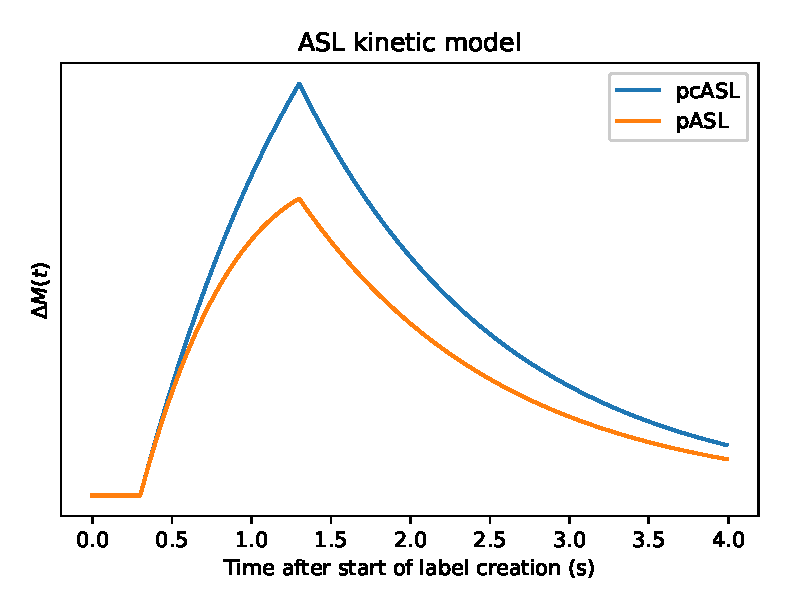
\includegraphics[width = 0.6\textwidth]{kinetic_curves.eps}
\caption{Kinetic models for pcASL and pASL with representative physiological and ASL parameters.}
\label{kinetic_curves}
\end{figure}

\subsubsection{Quantification with single- and multi-time imaging}

In light of the kinetic curves illustrated in figure \ref{kinetic_curves}, estimation of perfusion via ASL may be interpreted as a process of sampling different points on the idealised curves. The samples correspond to the subtraction of individual label-control pairs. Single-time imaging samples the kinetic curves at a single moment in time whereas multi-time imaging samples across multiple points in time (\textit{i.e.}, multiple positions on the $t$-axis). Although the former method is simpler, it naturally limits the number of parameters that can be estimated, whereas multi-time imaging allows estimation of both CBF and ATT. The difference between these two strategies is illustrated, along with the presence of acquisition noise, in figure \ref{single_multi_noisy}. 

\begin{figure}
\centering
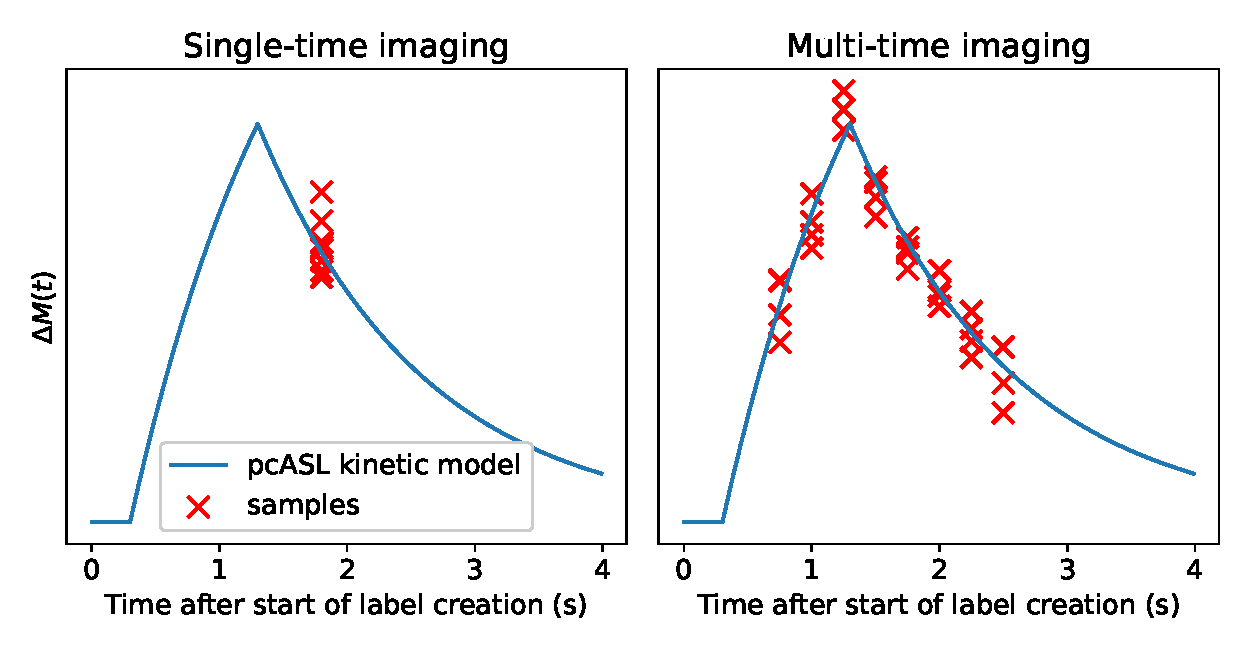
\includegraphics[width = 0.8\textwidth]{single_multi_noisy.eps}
\caption{Single- (left) and multi-time (right) imaging strategies. Multi-time better captures the shape of the kinetic curve and therefore allows for estimation of both CBF and ATT. For each case, the effect of white noise on the individual samples is shown. With sufficient samples, averaging at each sample time should yield the underlying signal value.}
\label{single_multi_noisy}
\end{figure}

\section{Parameter estimation via Bayesian inference}
\label{lit_vb}

In order to obtain parameter estimates (\textit{i.e.}, CBF, ATT, \textit{etc}) from physiological imaging data, it is necessary to \textit{fit} a model to the data. In the case of ASL, for which the kinetic model is non-linear, a widely used strategy is non-linear least squares fitting \cite{Chappell2009}. The drawbacks of such an approach are that it may not be robust in the presence of high noise, and that it does not allow for the incorporation of existing, or \textit{prior}, knowledge about what parameter values are plausible. 

An alternative approach to parameter estimation is based upon probability theory. The objective is to obtain a probability distribution on each parameter of interest. Such an approach acknowledges that, given acquired data, there are multiple values that each parameter could plausibly take, particularly in the presence of high noise. For example, in the case of the kinetic model for ASL, a high CBF and long ATT could be mistaken for low CBF and short ATT if one only had observations from a single moment in time; both are plausible parameter configurations given limited data. The advantage of using probability distributions on each parameter of interest is that it allows a `best' estimate, or most likely value, to be returned, as well as a measure of uncertainty on that estimate. 

There are two strategies for obtaining parameter estimates for a given model and acquired data. One approach deals with likelihood and answers the question \textit{what parameter values are most likely to produce the data that has been obtained?} The other approach deals with the posterior and answers the question \textit{given the data that has been obtained, what parameter values are most likely?} Though the difference is semantically subtle, there is an important mathematical distinction between the two that is readily be demonstrated via Bayes' theorem. Using the notation $y$ to denote the data that has been acquired (samples of the kinetic curve), $\theta$ to denote the parameters of interest (CBF, ATT, and potentially others), and $M$ to denote the generative model (the mathematical construct that maps $\theta$ to $y$, i.e., the kinetic model), an expression for the \textit{posterior} probability of $\theta$ is obtained as follows. 

\begin{equation} 
P(\theta | y, M) = \frac{ P(y | \theta, M) P(\theta | M) }{ P(y | M) }
\end{equation}

The term $P(y|\theta, M)$ is the \textit{likelihood} and is the focus of maximum-likelihood techniques, which make the assumption that the value of $\theta$ that maximises it will be approximately equal to the the value of $\theta$ at which the posterior is also maximal. However, two other terms modify the likelihood to give the posterior: the \textit{prior} $P(\theta | M)$ and \textit{evidence} $P(y | M)$. Because the evidence term simply acts as a linear scaling of the posterior (it is independent of the parameters $\theta$ that are sought), it is often neglected for simplicity. Similarly, because all terms have a dependence on $M$, it is often omitted from the notation for clarity. The posterior then becomes: 

\begin{equation} 
P(\theta | y) \propto P(y | \theta) P(\theta)
\label{eqn_bayes_posterior}
\end{equation}

This equation represents the basis of Bayesian inference methods. Note that when the prior is non-informative (represented by a uniform distribution), the posterior and likelihood terms will be linear mappings of each other (scaled by the evidence term); therefore likelihood and posterior based approaches are equivalent in this circumstance\footnote{For example, in the absence of any prior information, certain forms of Bayesian inference can be shown to be equivalent to non-linear least squares fitting \cite{Chappell2009}.}. 

There are three key advantages to using Bayesian inference over the more widely used maximum-likelihood methods. One is that it allows the incorporation of prior knowledge into $P(\theta)$ to guide the inference. The second is that it allows for an explicit treatment of acquisition noise (specifically, by incorporating it probabilistically into the generative model $M$). Finally, the inference process returns full parameter distributions as opposed to point estimates, which in turn enables the quantification of uncertainty on each parameter. For a technique that suffers from intrinsically poor SNR such as ASL, these features contribute to more robust parameter estimation. 

\subsection{Variational Bayesian inference}
\label{vb_section}

Although the equation underpinning Bayesian inference looks simple, in practice the technique can be difficult to implement analytically. This is because for all but the simplest models involving a low number of parameters and simple distributions, evaluating the posterior will entail performing an intractable computation. For example, if one wishes to ensure that the posterior is correctly scaled (all probability distributions should integrate to unity), then it is necessary to evaluate the evidence term $P(y | M)$ in the denominator of equation \ref{eqn_posterior_marginal}. This will entail the calculation of a marginal probability, as follows. 

\begin{equation} 
P(\theta | y, M) = \frac{ P(y | \theta, M) P(\theta | M) }{ P(y | M) }= \frac{ P(y | \theta, M) P(\theta | M) }{ \int_{\theta} P(y,\theta | M)P(\theta | M) \,d\theta }
\label{eqn_posterior_marginal}
\end{equation}

As the number of model parameters (dimension of $\theta$) increases, performing such integrations over a high dimensional space becomes infeasible. A number of approximative alternative strategies have therefore been developed, one of which is variational Bayesian (VB) inference. 

VB methods seek to approximate the true posterior using an arbitrary distribution $q(\theta)$, which itself is parameterised by a set of hyper-parameters (for example, $q(\theta)$ may be a normal distribution with corresponding mean and standard deviation, these latter quantities being the hyper-parameters). For \textit{each} parameter in $\theta$, there will be a corresponding distribution in $q(\theta)$ with a set of hyper-parameters. 

The quality of the approximation between $q(\theta)$ and the true posterior $P(\theta | y)$ may be quantified using the Kullback-Liebler (KL) divergence \cite{Wani2020}, defined in equation \ref{eqn_kl_div}. However, as calculating this quantity requires integration of the posterior $P(\theta|y)$ that is being sought in the first place, it cannot be directly evaluated. Nevertheless, with a quantitative measure of approximation quality thus defined, the inference process can be re-cast as an optimisation problem: what is the best approximation of the posterior, or, mathematically, \textit{what $q(\theta)$ minimises the KL divergence with the true posterior?}

\begin{equation} 
KL = \int q(\theta) \log{ \left[ \frac{ q(\theta)  }{ P(\theta|y) } \right] } \, d\theta
\label{eqn_kl_div}
\end{equation}

Minimisation of the KL divergence is equivalent to maximisation of a related quantity called the free energy \cite{Chappell2009}, defined in equation \ref{eqn_free_energy}. Crucially, all of the terms in this expression can readily be obtained: it is a function of the approximating posterior $q(\theta)$, the likelihood $P(y|\theta)$ and the prior $P(\theta)$. 

\begin{equation} 
F = \int q(\theta) \log{ \left[ \frac{ P(y|\theta) P(\theta) }{ q(\theta) } \right] } \, d\theta
\label{eqn_free_energy}
\end{equation}

This equation represents the objective of variational Bayesian inference: find the optimal $q(\theta)$ such that the free energy defined in equation \ref{eqn_free_energy} is maximised. Whilst it is not necessary to go into the mathematical details of how the optimisation is performed, a description of the process reveals the key assumptions that make this possible, and the restrictions they impose. 

\subsubsection{Mean field approximation}

In order to further simply the mathematics of VB inference, the mean field approximation is taken for $q(\theta)$. This entails splitting the parameters in $\theta$ into a number of independent subgroups $\theta_i$, which therefore means that $q(\theta)$ can be expressed as a product over the distributions of the individual subgroups. The practical impact of this is it reduces the number of terms that need to be calculated within the overall covariance of $q(\theta)$. A complete factorisation of all the individual parameters is not required \cite{Attias2000}. 

\begin{equation}
q(\theta) = \prod_i q_{\theta_i}(\theta_i)
\end{equation}

\subsubsection{Calculus of variations}

Maximisation of $q_{\theta_i}(\theta_i)$ over $F$ is obtained by applying the calculus of variations to yield a set of iterative update equations for the hyper-parameters of $q_{\theta_i}(\theta_i)$ \cite{Chappell2009}. The analytic form of these update equations follows from the choice of priors and likelihood that has been made. This is a crucial property of the VB framework and implies that if either the likelihood or priors are modified, then it is necessary to re-derive the update equations. 

The update equations for VB are generally not independent: the update for one $q_{\theta_i}(\theta_i)$ may depend on other $\theta_i$. As such VB follows the updating framework used by expectation-maximisation algorithms, in which the updates for all $\theta_i$ are performed using their values from the previous iteration, and so on until convergence.

\subsubsection{Conjugate exponential restriction}

In order to further simplify the derivation of the update equations on $q_{\theta_i}(\theta_i)$, a constraint on the form of the priors may be made such that they are conjugate with the likelihood \cite{Chappell2009}. This holds if and only if the prior is of the same parametric form as the posterior (for example, both being normal distributions). For reasons of tractability, distributions are often chosen from the exponential family and hence this aspect of VB is often referred to as the `conjugate-exponential' restriction. 

\subsubsection{Non-linear models; convergence}

VB as presented thus far applies to linear models (i.e., the data is a linear mapping of the parameters with some noise contribution). As demonstrated in section \ref{asl_kinetic_section}, obtaining parameter estimates from physiological imaging data can require fitting a non-linear model; the general kinetic ASL model is just one such example. It is possible to perform inference on non-linear models by approximating them with a Taylor expansion. The approximation may be weakly non-linear (Woolrich and Behrens used a second-order expansion \cite{Woolrich2006}) or may be fully linear (both Friston \textit{et al.} and Chappell \textit{et al.} used first-order expansions \cite{Chappell2009, Friston2007}). 

In general, the iterative updates derived under VB are guaranteed to converge as they are fundamentally a generalisation of expectation maximisation \cite{Attias2000}. The drawback of using approximations to fit non-linear models is that this guarantee is broken: as the inference is on an approximation of the model, not the model itself, convergence cannot be ensured in any region where the model deviates from the approximation. This is not an insurmountable problem and multiple authors have incorporated a `trial' process into their implementations of VB in order to spot convergence issues \cite{Chappell2009, Friston2007}. 

Chappell \textit{et al.}'s implementation of VB will be used multiple times throughout this work. Specifically, this consists of two tools included within FSL: FABBER is the core VB model-fitting algorithm, whereas BASIL is a wrapper around FABBER that facilitates ease-of-use for ASL applications \cite{Chappell2009, Chappell2011}. 

\subsection{The role of priors}
\label{vb_spatial_prior}

Priors play a central role in Bayesian inference. They can be used to convey the existence of prior knowledge about what values a parameter could take (for example, based on anatomy or physiology), or equally they can be used to convey the absence of knowledge (so called non-informative priors will not steer the inference process in any particular direction). Priors can also be defined in a spatial sense, \textit{i.e.}, with reference to the spatial distribution of parameter values. This is especially important in the context of neuroimaging as it allows the application of a near ubiquitous data-processing operation - spatial smoothing - in a principled manner. Smoothing is commonly applied to physiological imaging data in order to mitigate low SNR based on a two-fold assumption: firstly, that noise within the data is not spatially correlated, and therefore will be reduced by smoothing, and secondly, that the length scale of parameter variance will be relatively low compared to that of the smoothing kernel \cite{Jenkinson2017a}. The first assumption may readily be justified by knowledge of the acquisition process, but the second presents a challenge: the amount of smoothing to apply is ultimately at the discretion of the investigator and it will unavoidably obscure at least some spatial detail. 

Within a Bayesian framework, the key aspect regarding smoothing is the \textit{belief} on which the operation is justified: significant parameter variation is not expected between neighbouring voxels. This may be encoded using a Laplacian spatial prior. Conceptually, the Laplacian measures the curvature of a function and therefore returns high values for functions that are varying quickly in space. By interpreting the parameter values within voxels as samples from an underlying parameter field (for example, the `CBF' field), the Laplacian can be used to measure the local curvature for all voxel neighbourhoods. A neighbourhood containing many different parameter values is not smooth and such a configuration is probabilistically unlikely, or, in the terminology of the VB optimisation, will have a high latent cost. It is this cost that drives the optimisation towards more likely (spatially smooth) configurations. The benefit of incorporating this prior into the VB framework (a modification referred to as spatial-VB within FABBER \cite{Chappell2011}) is that that the weight that is given to the prior (the \textit{spatial precision}) is itself a target of the optimisation, which in turn negates the need for the user to specify this ahead of time \cite{Penny2005}. In practical terms, the degree of smoothing will be \textit{data-driven} and determined by how informative the data is. As will be discussed in section \ref{fabber_pvec}, spatial priors also enable partial volume effect correction to be performed. 


\section{Partial volume effects}

\subsection{Origin}

Physiological imaging techniques tend to use larger voxel sizes (around 3-4mm side length) than those used for structural imaging in order to improve SNR. As voxel sizes approach the length scale of structures of interest within the imaging region, individual voxels more are likely to intersect multiple structures and therefore contain a mixture of different tissues. The proportions of different tissues inside a given voxel are called partial volumes (PVs). In the context of brain imaging, the cortex is a structure of particular interest but presents a challenge because its mean thickness of 2.5mm in adults is approximately equal to voxel size \cite{Fischl1999a}.  

PVs give rise to a source of confound for the analysis of physiological imaging data because they pose a mixed-source problem: within each voxel, there are multiple sources (tissue types) but one measured signal (a sum weighted by the partial volumes of tissue in that voxel). This mixing is called the partial volume effect (PVE). It is desirable to know the physiological activity in each tissue separately; to do so it is necessary to un-mix the signal via partial volume effect correction (PVEc). 

PVE arise due to the highly specific interaction of a subject's anatomy, their location within an imaging matrix, and the imaging modality. Accordingly, for a given modality and imaging matrix, changes in subject anatomy over time will modify the distribution of PVE within the acquired data. This is especially the case for longitudinal studies of neurodegenerative disease such as Alzheimer's disease, which is characterised by the atrophy (thinning) of cortical GM regions \cite{Thompson2003}. For a given voxel intersecting such a region, the measured signal will decrease over time due to the reduced volume of cortex within that voxel. This introduces a source of negative bias into measurements, even though the tissue that \textit{does} remain in the voxel may be contributing proportionally the same amount of signal as before. Such a bias could obscure patterns that may be of interest when investigating biomarkers of disease \cite{Thomas2011}. 

\subsection{Partial volume estimation}

Any form of PVEc requires a set of PV estimates within the same voxel voxel grid as the physiological data as a point of departure. In essence, this is an explicitly volumetric representation of the problematic anatomy for which PVE have arisen. As this entails classification of the tissues (and their proportions) that are present in each voxel, this is closely related to image segmentation. It should be noted that PV estimates are specific to each acquisition, because they arise due to the acquisition-specific intersection of subject anatomy with the imaging matrix. 

Given the similarity with volumetric segmentation, many PV estimation techniques have used the same theoretical basis as segmentation methods. This includes Gaussian mixture model methods which treat the histogram of structural image voxels as the superposition of three individual Gaussian distributions corresponding to the dominant tissue classes (GM, WM, and CSF). The process of segmentation is then framed as determining to which distribution a given voxel is most likely to belong, based on its intensity. Santago and Gage provide a reference implementation of this approach \cite{Santago1993}. Though this concept can clearly be extended to PV estimation, there is a subtle difference between the two: segmentation aims to assign a \textit{single} label to a voxel, and therefore attempts to match it to a \textit{single} distribution, whereas PV estimation starts with the premise that there can be \textit{multiple} tissues present in a voxel. Furthermore, a 70\% chance of a voxel belonging to given tissue class does not necessarily imply that the voxel is 70\% comprised of that tissue, though some first-order relationship between the two could reasonably be assumed. A more direct treatment is to introduce explicitly mixed tissue distributions (\textit{e.g.}, GM and WM) into the framework, however due to the minimal divergence between multiple such distributions Santago and Gage found that the overall performance of this variant was worse than in the three-tissue case \cite{Santago1993}.

Despite their clear theoretical simplicity, mixture models, and more broadly histogram-based methods in general, face a fundamental challenge due to how PVE manifest themselves in the data. As illustrated in figure \ref{ideal_imperfect_pve_hists} on a simulated T1 anatomical image at high resolution, PVE can be thought of as increasing the within-class variance of samples drawn from an otherwise homogenous (low variance) tissue distribution. Visualised on a histogram, any amount of PVE is expected to lead to a broadening of the peaks that correspond to the pure distributions of each tissue. The challenge is that numerous other real-world effects also lead to the same outcome: for example, the presence of field inhomogeneities, acquisition noise and natural variability within tissue also increase the within-class variance of each tissue distribution (though many methods do attempt to account for these separately). Therein lies the difficulty: the basis in which mixture-model based methods seek to identify a partial volume voxel (the extent to which the voxel does not belong to any of the pure tissue distributions), is the very same basis on which other imperfections manifest themselves, leading to unavoidable ambiguity. In figure \ref{ideal_imperfect_pve_hists}, the idealised histogram corresponding to perfectly homogenous tissue distributions at high resolution is modified in two equivalent ways: firstly, by introducing high within-class variance but maintaining the same spatial resolution; and secondly, by introducing low within-class variance but also downsampling to reduce spatial resolution. Only in the latter case are PVE actually increased, but the outcome is similar in either case. 

\begin{figure}
\centering
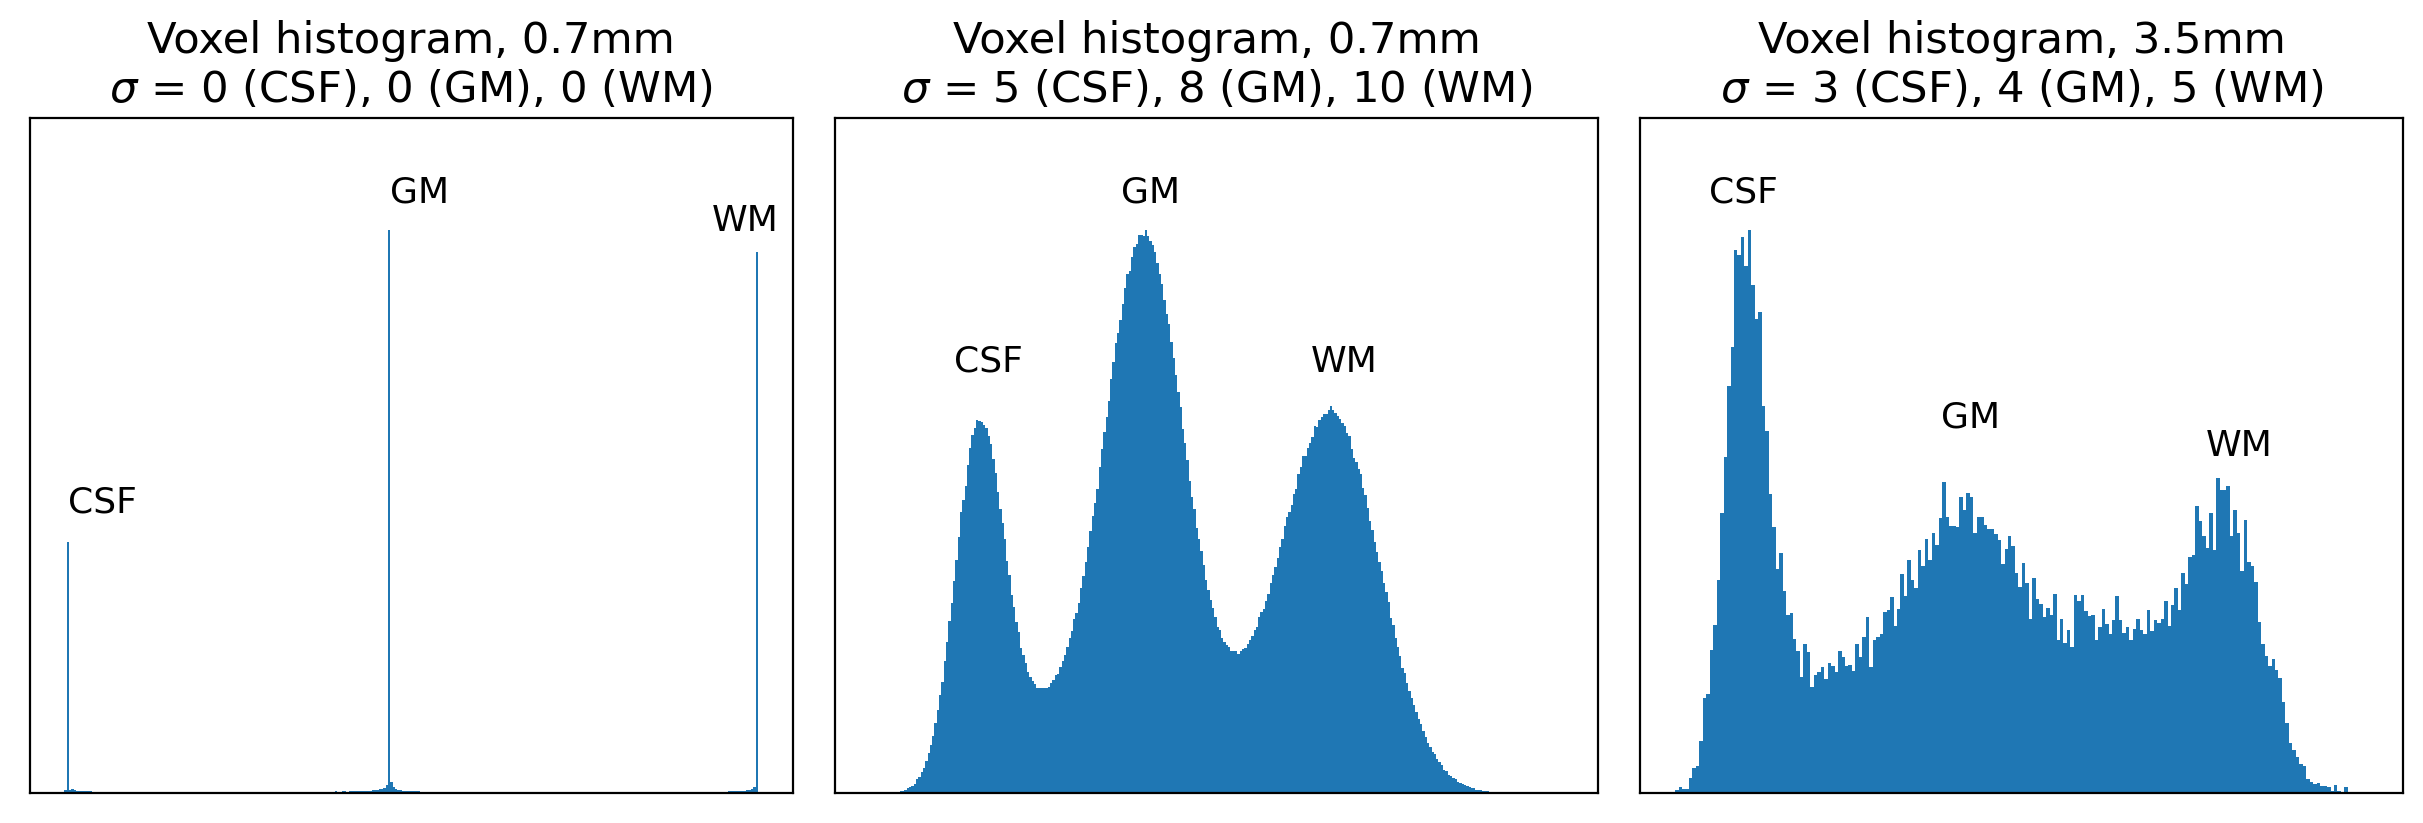
\includegraphics[width = \textwidth]{ideal_imperfect_pve_hists.png}
\caption{Left: voxel intensity histogram for a simulated T1 image at 0.7mm isotropic resolution with no within-class variance. Very few voxels contain PVs and therefore three sharp peaks are observed. Centre: histogram for a simulated T1 image at 0.7mm isotropic resolution, incorporating high within-class variance to represent real-world effects and imperfections. Numerous voxels lie in between the peaks corresponding to each tissue class. Right: voxel histogram for a simulated T1 image at 3.5mm isotropic resolution, with low within-class variance. Due to the much higher presence of PVE at low resolution, this histogram is similar in nature to the central plot; this demonstrates the difficulty of distinguishing PVE from other sources of variability.}
\label{ideal_imperfect_pve_hists}
\end{figure}

Segmentation and PV estimation techniques can also make use of spatial information in order to improve accuracy (so-called spatial mixture models). In keeping with the concepts presented in section \ref{vb_spatial_prior}, a spatial prior can be used to encode the belief that tissue classification should generally be homogenous across neighbourhoods of voxels, particularly if the length scale of voxels is small compared to the structures of interest (as is generally the case for structural MRI). FSL's FAST segmentation tool uses Markov random fields within an expectation maximisation framework to implement such an approach \cite{Zhang2001}. The same approach has also been implemented within a VB framework \cite{Woolrich2006}. The limitation of this strategy is that the belief it is founded upon - neighbourhoods of voxels should generally share similar classifications - is somewhat in contradiction to the very essence of PVE, namely that voxels may actually contain different tissues. A more fundamental point is the fact that the spatial prior is necessarily enforced in an isotropic manner at all locations within the brain. Deep within the large WM tracts of the subcortex, this is eminently appropriate, whereas at the deepest part of a sulcal pit, a sharp transition of tissue-type is expected and the assumption does not hold so well. 

The methods discussed thus far share the common property of being designed to work on structural resolution T1w images (though some also make use of the equivalent T2w images to exploit differing contrast). This is logical given that such images provide  high SNR, good tissue contrast and fine resolution for capturing spatial details. Accordingly, the PV estimates are returned in the same voxel grid as the anatomical image. For the purposes of PVEc, however, what is required are PV estimates in the same voxel grid as that of the data to be corrected, \textit{i.e.}, that of the physiological data. Resampling (a 3D interpolation operation) is therefore required to transform PV estimates from their native voxel grid to that of the physiological data. Due to the fact that the structural image may not be in alignment with the physiological data, a registration transformation may also be applied at the same time, so that the PV estimates are both transformed in space and resampled onto a new voxel grid; in either case, an interpolation is required. 

Due to the inherent resolution mis-match between structural MRI data and physiological imaging data, it is possible to derive PV estimates in the voxel grid of the physiological data using only a hard tissue segmentation (\textit{i.e.}, whole-voxel single-tissue labels). Because physiological imaging voxels tend to be much larger than structural voxels, each physiological voxel will enclose the same region of space as numerous structural voxels. A PV estimate for the larger voxel can therefore be obtained by simply counting the individual tissue labels of the corresponding structural voxels, without needing to explicitly perform PV estimation on the original structural data. Resampling tools such as FSL's \textit{applywarp} perform this summation over voxel neighbourhoods when dealing with mis-matched resolution data in order to better capture PVE \cite{Andersson2010}. The PVEc tools included with PETSurfer also derive their PV estimates in this manner \cite{Greve2016}, namely via FreeSurfer's binary segmentation at structural resolution.  

The method introduced by Ahlgren side-steps the need for resampling entirely by estimating PVs in the native space of an ASL acquisition \cite{Ahlgren2014}. This is achieved via the use of a T1-mapping approach applied to ASL data obtained via a QUASAR sequence. Because both the PV estimates and the ASL data to be corrected are derived from the same acquisition, there is no need to perform a registration or transformation, which therefore removes the possibility of this step introducing error. Unfortunately, this approach is restricted to use only with QUASAR data and the segmentation algorithm used is simplistic. 

\subsection{Correction methods}

Due to the fact that both ASL and PET suffer from PVE (in slightly different forms), numerous correction strategies for both modalities are reported in the literature. Examples of both will be given here. 

As PVE are an example of a mixed-source problem, they naturally lead to an under-determined system of equations within each voxel. Neglecting any signal contribution from CSF (which is assumed to be inactive), the physiological activity $S$ in a voxel may be expressed as a linear sum. 

\begin{equation}
S = P_{GM} F_{GM}+ P_{WM} F_{WM}
\end{equation} 

$P_t$ is the partial volume of tissue $t$ within the voxel and $F_{t}$ the physiological activity associated with that tissue in isolation. There are infinitely many solution pairs of $F_{GM}$ and $F_{WM}$ that satisfy this equation; PVEc methods differ in how they select a single pair.

\subsubsection{Linear regression}

Linear regression (LR) methods assume that perfusion within GM and WM are constant within a 2D or 3D kernel of side length $n$, containing $N$ voxels in total, centred at the voxel in question (the kernel may include only direct neighbours, or first diagonals, \textit{etc}). Under that assumption - a spatial prior of local similarity - the equation can be expressed in matrix form as

\begin{equation}
\vec{s} = \mat{P} \vec{f^*}
\end{equation} 

where $\vec{s}$ is a vector of length $N$ containing individual voxel signals, $\mat{P}$ is a matrix of size $N$ x 2 containing PV estimates for the kernel, and $\vec{f^*}$ is a vector of length 2 containing the GM and WM parameter values of interest. This equation may be solved for $\vec{f^*}$ with the pseudo-inverse of $\mat{P}$ which is equivalent to a least-squares linear regression solution. The major drawback of this approach is the smoothing effect imposed by the assumption of constant perfusion within the kernel, the extent of which is determined by the kernel size. Given the poor spatial resolution of physiological imaging data, and the length scale of structures of interest in the brain, this approach poses a risk of smoothing over important detail in structures such as the cortex. Asllani provides a reference implementation of this method for ASL data \cite{Asllani2008}. 

Petr \textit{et al.} investigated an extension of the LR method \cite{Petr2010}. They approached the problem as one of noise reduction via smoothing (the inevitable consequence of performing linear regression over kernels). Their key contribution was to constrain the smoothing operation to minimise signal variation within tissue classes whilst avoiding mixing signal \textit{between} classes and respecting regional variations in perfusion. The authors argued that this would make it more appropriate than standard LR for cases of pathology where local anomalies in perfusion need to be detected. 

A further extension of LR was developed by Liang \textit{et al.} \cite{Liang2013}. Again addressing the problem of smoothing imposed by the assumption of constant CBF over spatial kernels, the modified trimmed least squares (mTLS) approach essentially seeks to perform outlier rejection when constructing kernels within each voxel neighbourhood. The smoothing imposed by LR is most severe when the voxels within a neighbourhood have very different values. Accordingly, mTLS iteratively constructs kernels that include only the most similar voxels to the one currently undergoing correction. The authors reported reduced smoothing and better preservation of details, especially around the edges of structures. The method does require one user-set parameter, though the optimal value for this has been determined empirically on both simulations and \textit{in-vivo} data. 

\subsubsection{Spatial-VB}
\label{fabber_pvec}

Spatial-VB sits within FABBER's implementation of VB for ASL, presented in section \ref{vb_section}. Rather than fitting a kinetic model for a single tissue to the data (with a single CBF, ATT, T1 value \textit{etc}), a model with separate components for GM and WM is fitted in proportion to the PV estimates present in each voxel\footnote{This is a two step process, with an initial fit performed in single-tissue mode that is used as the basis for a second fit in both GM and WM. In each case, the FSL tool BASIL uses FABBER to perform the fit.} \cite{Chappell2011}. In this circumstance, the spatial prior introduced in section \ref{vb_spatial_prior} plays a dual role. Whereas previously it was used to enforce similarity between voxels as a means of performing noise rejection, in this situation it also \textit{conditions} the inference problem. This means that it allows for the inclusion of neighbourhood voxels in order to solve the inherently under-determined system of equations that arise due to PVE. In practical terms, this is equivalent to assuming constant parameter values across the neighbourhood of voxels, as is the case for LR, but crucially the strength of this assumption is relaxed compared to the LR case. This is because the weight given to the prior is a property of the optimisation itself, determined from the data, which generally results in reduced levels of smoothing compared to LR. A somewhat counter-intuitive feature of this approach is that it entails fitting components for GM and WM in all voxels, regardless of which tissues are actually present. For example, in the case of ASL, this means GM CBF and ATT will be estimated even in voxels that do not contain any GM. Though seemingly paradoxical from an anatomical point of view, the situation may be thought of in terms of fields: there exists a GM CBF field across the entire brain, from which samples are drawn at specific locations where the GM PV is non-zero, and in other voxels the spatial-VB approach will interpolate in value derived from informative neighbours. 

\subsubsection{PETSurfer}

PETSurfer is a subset of tools embedded within FreeSurfer (introduced in section \ref{surface_segmentation}) for kinetic modelling and PVEc of PET data \cite{Greve2016}. The nature of PVEc for PET is slightly different than for ASL due to spill-in / spill-out effects. These arise due to the relatively high point-spread function (PSF) of PET data compared to the voxel size used for imaging; the voxel in which signal appears is thus not necessarily the same as that where the signal was created. In fact, the partial volume effect that arises due to the presence of multiple tissues within a voxel is referred to in the PET literature by the alternative name of tissue fraction effect (TFE); Erlandsson discusses these differences in greater detail \cite{Erlandsson2012}. Three PET-specific PVEc methods are implemented within PETSurfer: Meltzer (MZ), Muller-Gartner (MG), and symmetric geometric transfer matrix (SGTM); all of which attempt to deal with PSF issues in different ways. The former two methods can be used for voxel-wise analysis whereas the latter is restricted to region-of-interest analysis only. 

The MZ method addresses only the PSF effect and does not attempt to separate out tissue contributions \cite{Meltzer1990}. For ASL, the PSF is of lower importance and the TFE is the key driver of PVE. As part of the correction, the user is required to set a manual PV threshold on voxels at the edge of the brain (usually in the region of 10 - 50\% tissue). 

The MG method addresses the PSF effect and attempts to remove the contributions of WM and CSF to leave a pure GM signal \cite{Muller-Gartner1992a}. This is achieved by deriving a single global value for WM and CSF contributions (using appropriately drawn ROIs), subtracting this value from mixed voxels, and finally scaling the remaining signal to account for lost tissue volume. The assumption of a single global value for WM and CSF is clearly of high importance; the same could not necessarily be made of other modalities. Once again the user is required to set a manual threshold on voxels to exclude from the correction. 

The SGTM method \cite{Labbe1998} is conceptually similar to the LR method for ASL: a linear matrix system that relates signal in a set of ROIs to voxel values is formed. 

\begin{equation}
\vec{y} = \mat{X}\vec{\beta}
\end{equation}

$\mat{X}$ is the key construct that maps individual voxels to their respective ROIs in a manner that accounts for both PSF and TFE; $\vec{y}$ and $\vec{\beta}$ are voxel-wise data and the desired ROI signal values respectively. Because $\mat{X}$ is dependent on the PSF it may be badly conditioned (leading to noise amplification) or non-invertible \cite{Greve2016}. 

Though in principle these methods could be made to operate with other modalities, they would require some degree of manual tuning for optimal performance. Although SGTM has performed favourably in comparison studies \cite{Greve2016}, the fact that it does not permit voxel-wise analysis would be a significant hinderance for a modality such as ASL, where volumetric analysis is increasingly widespread\footnote{Often, ASL studies simply report overall CBF values within regions of interest as opposed to voxelwise maps. Nevertheless, the underlying parameter estimation required to obtain such summary statistics is volumetric in nature, \textit{i.e.}, mathematical operations on voxels of data.}.

\subsubsection{Impacts of PVEc}

Numerous authors have investigated the consequences and benefits of performing PVEc. Evidence from both the PET and ASL literature suggests that there are important analysis benefits that can be realised with PVEc, but careful decisions must be made about the methods used (and the assumptions they encode), especially for methods that require user-set parameters. Nevertheless, in spite of these risks, a soft consensus is emerging that the difficulties of performing PVEc are not sufficient to disqualify the operation entirely. 

Erlandsson's review of PVEc methods for PET concluded that it is an ``important aspect'' of quantitative analysis, though also lamented the lack of existing ``turn-key'' solutions. This lack was attributed to the various methodological challenges and implications that are posed by PVEc: a high reliance on accurate segmentation and registration (particularly between MRI and PET data), potentially high sensitivity to noise, and the difficulty of justifying the assumptions that are required \cite{Erlandsson2012}.  

More recently, Greve \textit{et al.} investigated correction of a PET ageing dataset and found that, in the absence of PVEc, the data was ``highly contaminated'' by anatomical changes; a bias that was successfully removed with PVEc \cite{Greve2016}. SGTM was reported favourably as it required the fewest assumptions and was the most robust, though at the cost of permitting ROI-based analysis only. They also reported a diversity of results across different PVEc methods, which they conclude ``mirrors the confusion found in the literature about ageing and metabolism'' \cite{Greve2016}. 

Thomas \textit{et al.} found PVEc to improve the quantitative accuracy of amyloid PET regional analysis \cite{Thomas2011}. Some of the assumptions made by PET-specific strategies were found to introduce biases that lead to erroneous inferences, though this was not the case for the more recent methods. As applied to a multi-subject dataset, PVEc increased inter-subject variability, though the authors believed the increase to be genuine, leading them to conclude that PVEc should be mandatory in clinical studies in consequence of the improved accuracy it offers. Taken together, the findings of both Thomas \textit{et al.} and Greve \textit{et al.} highlight the fact that successful PVEc requires careful consideration of the context-specific biological and technical factors that give rise to PVE \cite{Thomas2011, Greve2016}. 

For ASL, Petr \textit{et al.} \cite{Petr2018} investigated the accuracy of PV estimates derived from T1w images for the application of different forms of PVEc (including quasi-methods, such as simple thresholding over ROIs). Whilst they did find geometric distortion and differences in effective resolution between ASL and structural data introduce some error into CBF quantification, this was not a sufficient basis to abandon PVEc altogether: ``PVEc remains the most accurate way to calculate GM CBF''. Furthermore, they found the differences arising due to the ASL-T1w mismatch to be of similar magnitude to the effect sizes in many CBF studies, thereby emphasising the importance of PVEc as a means of increasing statistical power. 

A separate investigation by Petr \textit{et al.} on their extension of the LR PVEc method reported increases in SNR for acquisitions with less than 20 label-control repeats, though SNR decreased above this number (because the extra signal imparted by more repeats outweighs the loss of signal caused by excessive smoothing) \cite{Petr2010}. 

An evaluation of the LR and spatial-VB PVEc methods for ASL showed that spatial-VB better preserves spatial details than LR at the cost of higher sensitivity to noise \cite{Zhao2017a}. Both methods were shown to reduce inter-session variability (this is especially important for longitudinal studies). PVEc of either form was also shown to be sensitive to errors in the PV estimates themselves. 

Despite the evidence that PVE present a significant challenge for quantitative analysis of ASL, PVEc remains rare within clinical studies that make use of this modality (a methodological review performed in 2017 found that 5\% of clinical studies explicitly reported performing this step\footnote{A sample group of 39 studies was assembled in the following manner. Firstly, a search on Scopus for \textit{( ( asl OR “arterial spin labelling” ) AND ( “functional” OR “fMRI” ) AND “clinical” AND ( “brain” OR “cerebral blood flow” OR “CBF” ) ) year $\geq$ 2010} yielded 236 papers that were sorted by number of citations and the top 28 that contained experimental work with a clinical endpoint. To these were added 11 papers from the monthly ASL Network newsletter, drawn from the section \textit{cerebral blood flow studies; studies on special disease} and also having a clinical endpoint.}). Indeed, the recommended implementation for ASL in clinical use merely highlights PVE as a source of confound without addressing how PVEc should be performed \cite{Alsop2015}. 


\section{The surface paradigm}

Volumetric imaging techniques necessarily divide the imaging region into discrete subunits called voxels. Signals are aggregated within these voxels with no regard to the underlying anatomy (or anatomies) that have produced them. Finally, the data arising from such an acquisition is represented using a three or four dimensional matrix structure that matches the discretisation of space. Surface representations of data stand in contrast to this. Instead of discretising the imaging region into regular volume units, surface methods assume that signal originates from discrete areas lying on some topological plane (which may nor may not be closed). A basic assumption that underpins the surface approach holds that locations on a surface will correlate better according to geodesic distance (along the surface) than geometric (straight-line). For example, on the cortical surface, areas on opposite sides of a sulcus are close in a geometric sense but distant in a geodesic sense. Electroencephalography (EEG) provides a useful discussion point to illustrate the key concepts. 

EEG is concerned with electrical activity within the cortex. Electrodes are distributed across the scalp in a known configuration. Conceptually, the signal generation and acquisition system may be thought of as two concentric spheres with differing radii: the cortex lies inside the sphere defined by the electrodes, and the small distance between them is taken up by the cranium and CSF (which have some transfer function that maps cortical activation to observed signal at the electrodes). 

Given how the signal is generated and acquired, it would be illogical to try and represent the signals recorded by the electrodes in a volumetric manner, whereas a surface representation lends itself readily. This is not without challenges (for example, source reconstruction, the localisation of individual activations on the basis of their appearance at multiple electrodes simultaneously, is complex), but the representation of the data naturally fits the anatomy of the structure of interest. 

Although volumetric imaging techniques such as PET and MRI cannot readily be made to operate in a surface-based manner, it is possible to process, transform and analyse the data they produce in such a way. In order to do so, a number of building blocks are required: a means of generating the surfaces of interest (surface segmentation), a means of moving data from a volumetric to a surface representation (surface projection), and finally a means of analysing data on the surface (surface-based analysis). 

\subsection{Surface segmentation}
\label{surface_segmentation}

Segmentation in a volumetric sense involves assigning class labels to individual voxels, themselves the discretisation basis of the imaging region, so the process is inextricably linked to the voxel grid of the image itself. Surface-based segmentation is independent of the voxel grid of the data on which it is performed. The segmentation aims to identify the boundaries between different regions of tissue within the image, which are modelled as contiguous triangular meshes, the vertices of which are calculated with sub-voxel (i.e., continuous) precision. This is in contrast to volumetric segmentation in which boundaries are necessarily identified with whole-voxel (discrete) precision. 

Surface segmentation also allows for the incorporation of spatial and geometric constraints informed by anatomy. For example, FreeSurfer - a tool that enjoys especially widespread support within the literature - segments the cortex according to the principle that it lies in between two contiguous (topologically spherical) surfaces, one defining the WM/GM boundary and the other the GM/CSF boundary \cite{Fischl2012}. Example FreeSurfer surfaces are shown in figure \ref{fs_demo}. FSL FIRST uses shape-based models as priors to segment subcortical structures \cite{Patenaude2011}. Tissue continuity is enforced anisotropically in either case: the premise of surface segmentation is that tissue is homogeneous \textit{along} a surface but heterogeneous \textit{across} it. This contrasts with the spatial prior used by FSL FAST, for example, which is necessarily enforced isotropically, \textit{i.e.}, with no regard for the underlying anatomy. 

\begin{figure}
\centering
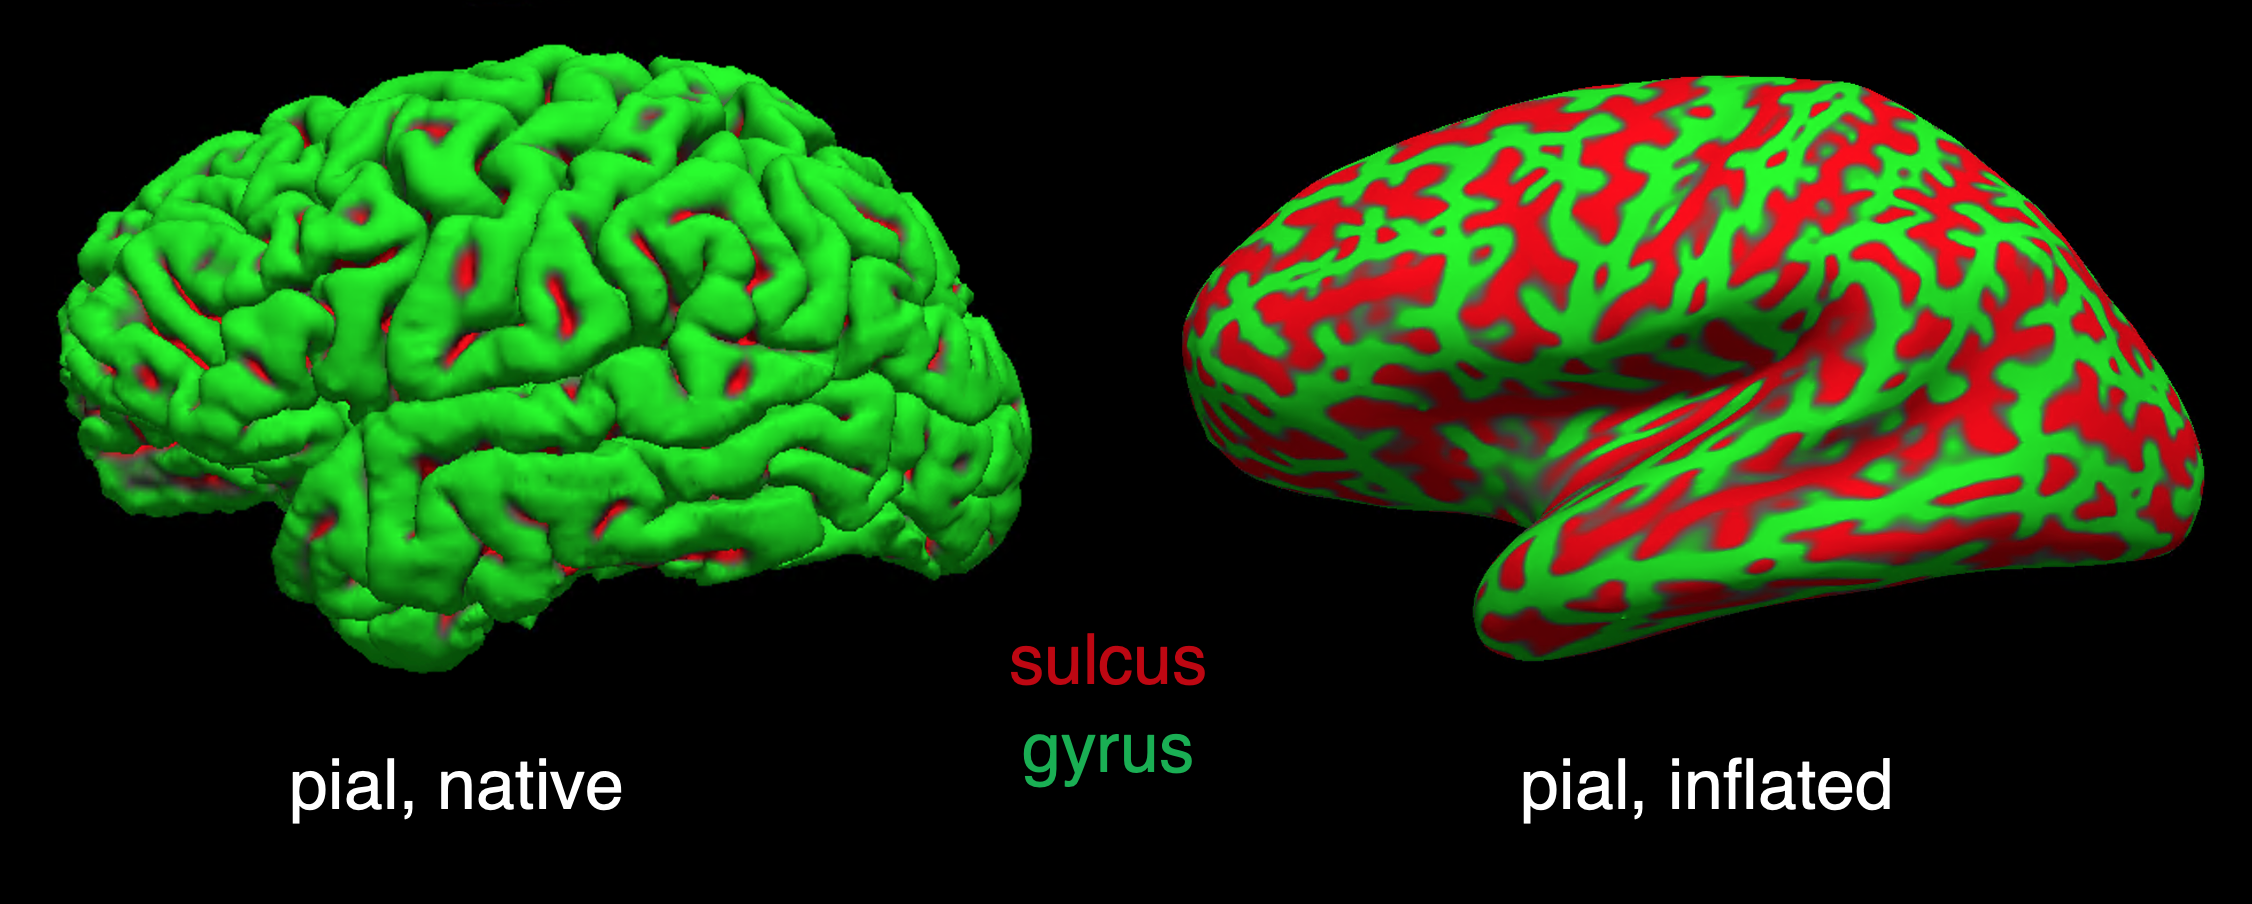
\includegraphics[width=\textwidth]{fs_demo.png}
\caption{Example FreeSurfer segmentations of the pial (outer) surface of the cortex. Both the native and inflated surface are shown; as there is vertex correspondence between the two, the inflated surface can be used to visualise data that would otherwise be obscured at the bottom of sulcal pits (highlighted in red).}
\label{fs_demo}
\end{figure}

Whilst the objective of surface segmentation is conceptually clear, there is a degree of subjectivity to it from an anatomical point of view: the notion of a hard border between WM and GM in the cortex is artificial and reality is better described by a gradient transition, albeit over a short length scale \cite{Dale1999}. Though it is difficult to determine with certainty whether surface or volumetric segmentation methods are more accurate for the cortex – defining an unambiguous ground truth for brain segmentation is challenging \cite{Shattuck2009} – the aforementioned characteristics of the surface-based approach suggest it is theoretically better suited to segmenting the cortex and it is well-established within the literature for this purpose. 

 
\subsection{Surface projection}
\label{lit_projection_methods}

Data that has been acquired in a volumetric manner must be transformed `onto the surface' before it can be analysed in that space. This is a complex transformation for which there is no single analytic solution (consider, for example, the change in dimensionality from 3D to 2D that is necessarily entailed). 

Prior work for the projection of MRI data has largely addressed BOLD fMRI and is constrained to the cortex. Grova \textit{et al.} \cite{Grova2006} approached the problem as one of interpolation: projecting data onto the surface may be thought of as equivalent to interpolating signal from a regular grid of voxels onto surface vertices. Their contribution was to incorporate anatomical constraints into the interpolation kernels, achieved by defining the kernels around each vertex in terms of Voronoi regions grown within the cortical ribbon instead of the more-commonly used spherical kernels. This has the advantages of ensuring that all cortical voxels contribute signal to the interpolation operation (which would not be the case for spherical interpolation) and minimising the number of voxels shared between neighbouring interpolation kernels. This approach was also found to be insensitive to the specific locations of surface vertices within the cortical ribbon and to be robust to registration error. This method does not explicitly define a reverse projection. 

The ISA method developed by Lonjaret \textit{et al.} \cite{Lonjaret2017} approaches the problem from the inverse direction. A model is constructed that maps cortical activations to volumetric data, incorporating knowledge of the BOLD signal mechanism and partial volume effects. The model may be expressed as a single matrix multiplication of the form 

\begin{equation}
\mat{V = M \Gamma}
\end{equation}

where $\mat{\Gamma}$ represents timeseries data on the cortical surface, $\mat{M}$ the surface-to-volume projection matrix and $\mat{V}$ the timeseries of voxel data. The volume-to-surface projection is then performed by approximating the solution to the inverse problem, \textit{i.e}., solving for $\mat{\Gamma}$. At typical fMRI resolution, there will be multiple surface vertices in each voxel, leading to a highly under-determined and ill-conditioned system (within each voxel, multiple different vertex values can be combined to give the same overall value). As such, their solution makes use of prior knowledge of the BOLD signal and empirically-determined regularisation terms to guide the solution. This means that it is not readily applicable to other modalities in its native form and would first require specific tuning. 

The ribbon-constrained (RC) method developed by Glasser \textit{et al.} \cite{Glasser2013} as part of the HCP also incorporates anatomical constraints by operating entirely within the bounds of the cortical ribbon, as defined by the inner (white) and outer (pial) surfaces of the cortex. Vertex correspondence between the two surfaces is exploited to construct polyhedra lying within the cortical ribbon. Voxels in the surrounding neighbourhood are tested to determine their volume of intersection with each polyhedron, the values of which are recorded. The projection is then performed as a weighted-averaging operation, with the individual weightings of each voxel to each polyhedra calculated from the volumes of intersection. The reverse projection is also well-defined for this method and may be constructed from the same principles.

None of the aforementioned projection methods discriminate between signal that is cortical or non-cortical in origin. This raises the possibility that signal originating in the subcortex may in fact be projected onto the cortical surface, introducing error or bias into subsequent analysis. By and large, this situation is treated as a problem to be addressed separately (for example, by attempting to regress out subcortical signal once in the surface space). In fact, developing a projection framework that could discriminate between cortical and subcortical signal would be a substantial challenge: in essence, this would imply the simultaneous application of PVEc which is a non-trivial operation. 

\subsection{Surface analysis}

Of all of the constituent parts of a surface-based approach, the choice of analysis method is the most open-ended as it is highly specific to the data and modality in question. Numerous methods have been developed for both structural and physiological imaging data. 

For structural data, the geometry of surface segmentations provides a wealth of useful data. Measurements of cortical volume and thickness can readily be obtained from a set of cortical surfaces \cite{Fischl1999a}; these have been shown to be indicative of a variety of pathologies including neurodegeneration \cite{Harvey1993, Rimol2012, Knopman2016, Lin2017}. The extent and depth of cortical folds (sulci and gyri) is a marker of neurodevelopment \cite{Tamnes2017, Garcia2018} and their locations are useful predictors of functional arrangement \cite{Fischl2008}. Folds have also been used as a basis for performing inter-subject registration between surfaces \cite{Lyttelton2007}, although in isolation they do not necessarily provide optimal alignment of functional sub-regions \cite{Robinson2013}. 

For physiological data, surface-based analysis of has been shown to reduce bias and variance in the kinetic modelling of PET data \cite{Greve2014}. In that work, the reduction in inter-subject variance observed was sufficient to reduce the number of subjects required to achieve a given level of statistical power by a factor of four. This result was obtained by applying a combination of PVEc and smoothing constrained to apply only along the surface; both operations seek to minimise mixing of signal between heterogenous tissues, leading to substantial increases in the detectability of effects. Verclytte \textit{et al.} \cite{Verclytte2015} analysed an ASL dataset of early-onset Alzheimer's disease patients via projection onto the cortical surface. This was an early example of surface-based analysis for ASL data, although only the final CBF maps were projected (all quantification, including PVEc, was performed volumetrically). 

Surface-constrained smoothing contrasts with conventional volumetric smoothing, in which signal is mixed with no regard to underlying structure (\textit{i.e.}, both on and off the surface). Some have taken the principle further by integrating surface parcellations into the process; the result is smoothing that is constrained within functionally similar areas of cortex, further reducing the mixing of dissimilar signals. The HCP is a notable proponent of this approach \cite{Glasser2013, Coalson2017}. Mathematically, surface constrained smoothing requires the calculation of geodesic (along the surface) as opposed to geometric (straight-line) distances when evaluating the weights of the smoothing kernel. 

Surface analysis provides further advantages for multi-subject and multi-modal studies. Conventionally, a non-linear volumetric registration is used to establish spatial correspondence between multiple subjects, after which physiology and functional correspondence are investigated. As non-linear registration is a highly complex operation with no unique solution, it can be an important source of error, or loss of statistical power, in the subsequent analysis. This is particularly true at the very fine length scale of the cortex, for which significant natural variability of anatomy across a population is expected. This variability can be seen on the MNI152 1mm standard brain, illustrated in figure \ref{mni152}. This standard is constructed by non-linearly registering and averaging a T1w structural image across multiple subjects; accordingly the subcortex appears very homogenous (all subjects have WM in approximately the same place), whereas the cortex is blurred because the precise location of sulci and gyri amongst subjects is less certain. 

\begin{figure}[h]
\centering
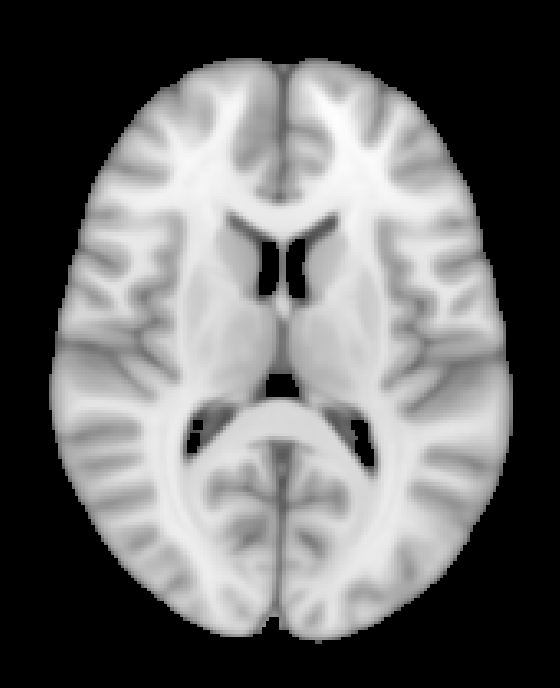
\includegraphics[width = 0.4\textwidth]{mni152.png}
\caption{The MNI-152 standard brain at 1mm resolution. Due to the nature of its construction (which involves averaging across many subjects), structures which are consistently located across subjects (\textit{i.e.}, WM tracts) appear homogenous, whereas regions such as the cortex that are highly variable between subjects are blurred significantly.}
\label{mni152}
\end{figure}

Even when regions of functional correspondence can be established under a conventional volumetric approach, Coalson \textit{et al.} argue that they are ``little more than statistically significant blobs” whose precise relationship to anatomy is uncertain \cite{Coalson2017}. In essence, this situation arises because volumetric registration is performed on the basis of anatomy, but this does not guarantee that areas of function (the ultimate objective) will also align, because the function-anatomy relationship for individual subjects is uncertain. 

Surface-based methods provide an alternative approach. As adopted by the HCP, inter-subject registration can be performed by aligning cortical areas using both folds and `areal' features such as cortical myelin content and resting state networks. Importantly, these features are more closely related within the boundaries of said areas than structural image intensities in volume space \cite{Glasser2016a} or cortical folding patterns \cite{Robinson2014, Robinson2018}. This approach is named multi-modal surface matching (MSMAll) and is able to fuse information from multiple modalities \cite{Robinson2013}. The literature shows there is a clear improvement in the accuracy of inter-subject correspondence of functional areas over volumetric registration under this approach. For example, standard volumetric methods achieved just 35\% of the spatial localisation accuracy of the MSMAll method as used on HCP data \cite{Coalson2017}. A comparison of inter-subject registration based on folding alone versus MSMAll is shown in figure \ref{msmall_demo}.

\begin{figure}[H]
\centering
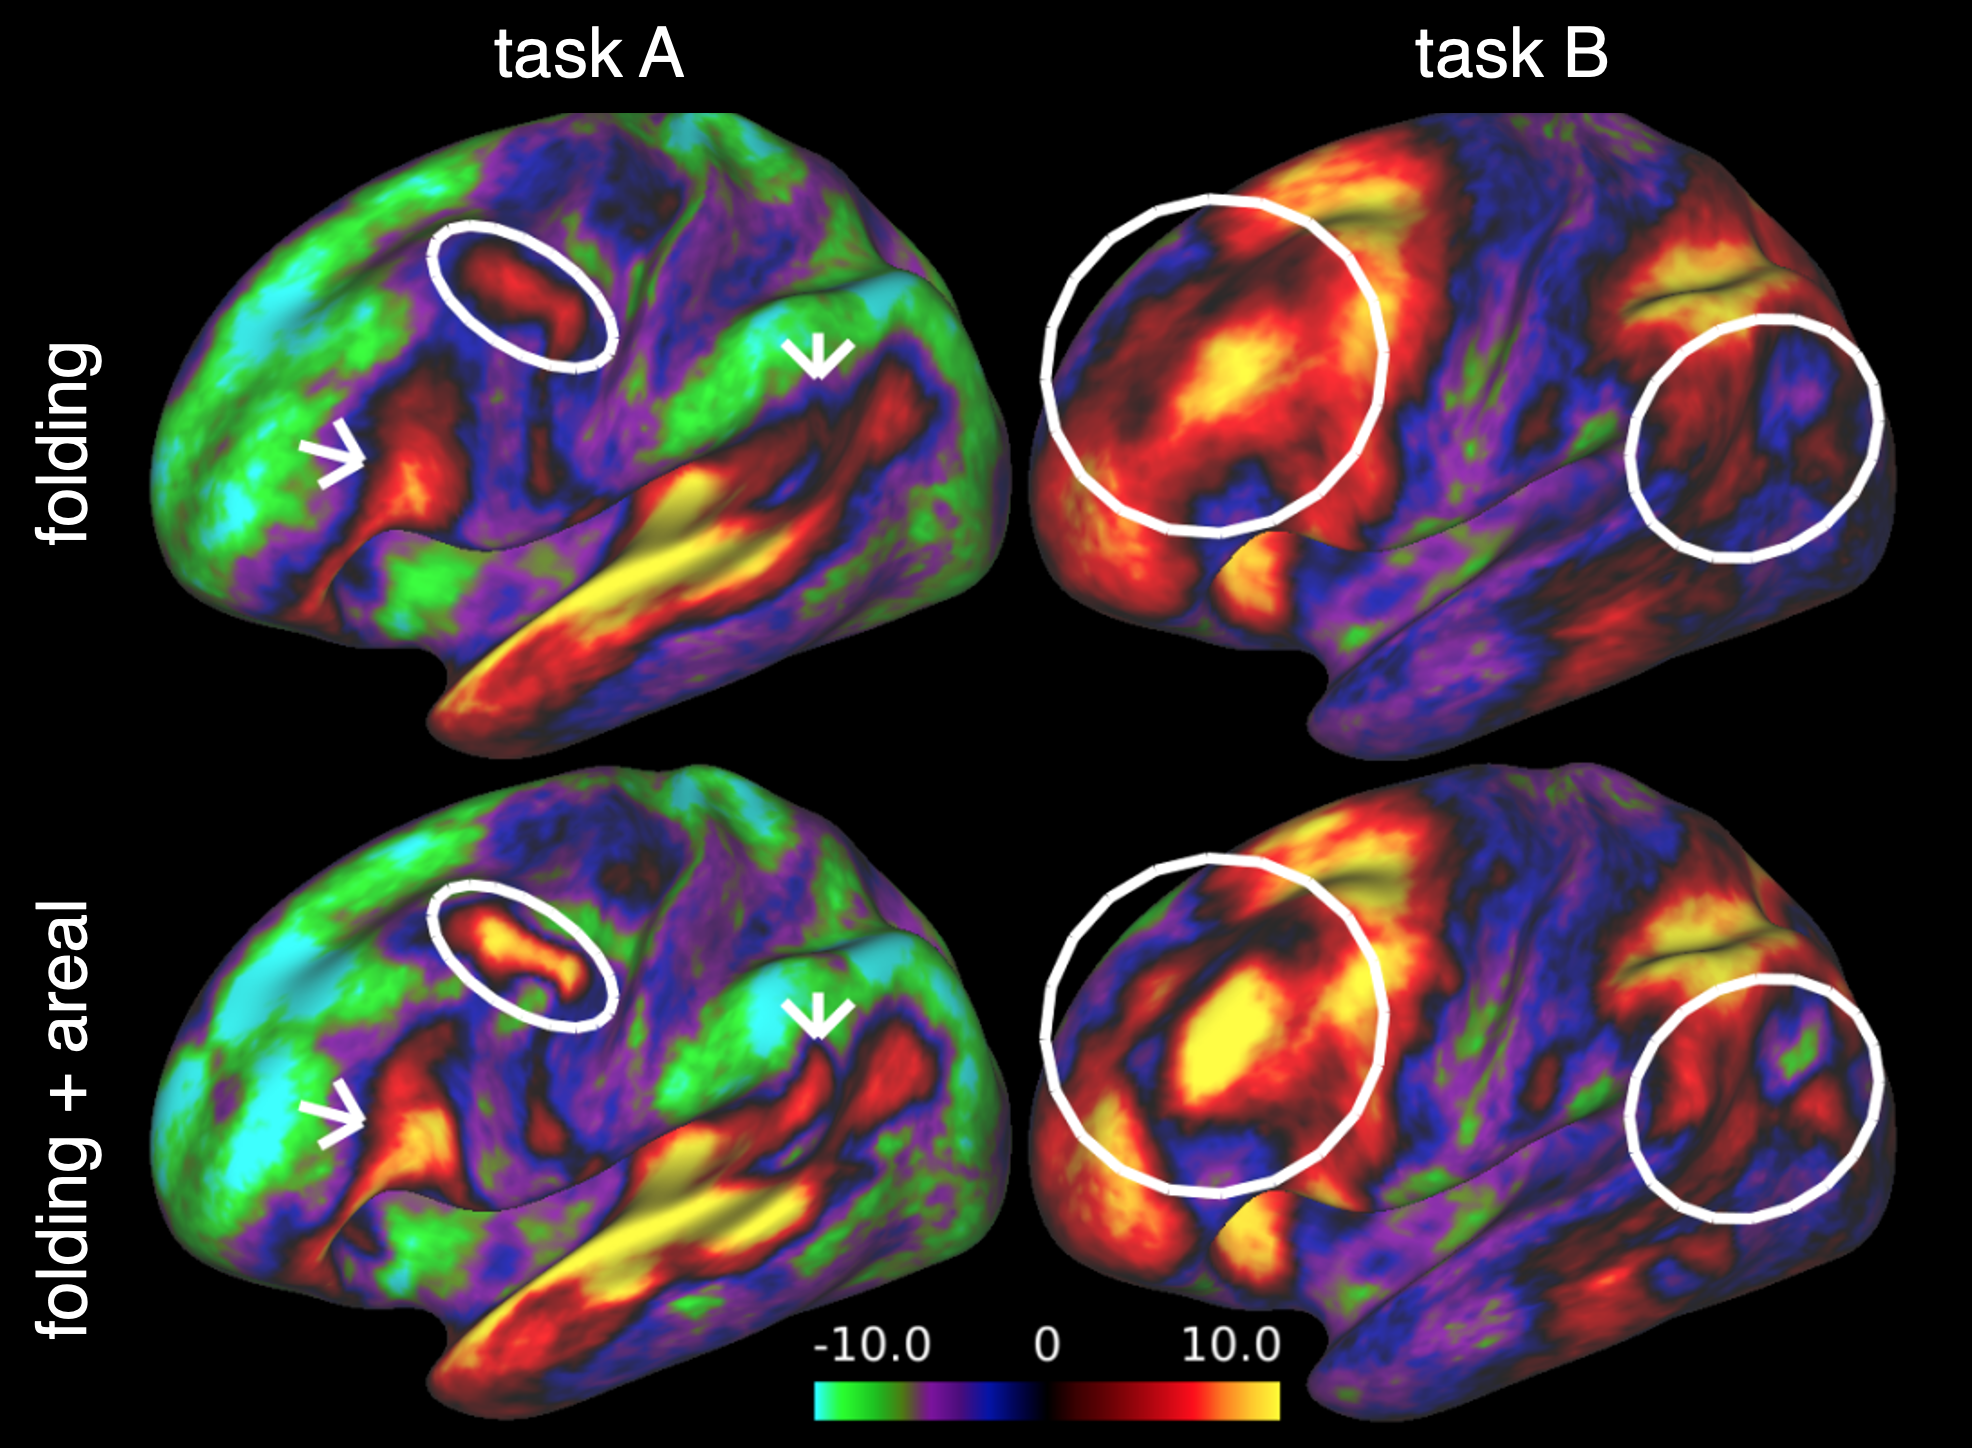
\includegraphics[width = \textwidth]{msmall_demo.png}
\caption{Comparison of surface registration across 120 subjects from the HCP. The top row shows registration based on cortical folding only, whereas the bottom row shows registration based on both folds and areal features (MSMAll). The columns show two different fMRI tasks and the data plotted on the surfaces are the group average $Z$-statistics. MSMAll registration results in increased contrast which is indicative of improved functional correspondence across subjects. Circles and arrows highlight areas of particular difference. Reproduced with permission from \cite{Glasser2016a}.}
\label{msmall_demo}
\end{figure}


\section{Summary}

The aim of this review has been to introduce two broad themes. The first of these, PVE, are an unavoidable consequence of imaging complex anatomies with techniques that have limited spatial resolution. They present an important and widely acknowledged source of confound across multiple modalities and remain a problem for which there is no consensus solution. The importance of this issue is increased when it is desired to study structure and function simultaneously and longitudinally, for example when investigating the structural and physiological changes that accompany brain disease. 

The second theme is the emergence of a surface-based analysis paradigm for the study of the cortex, which has bought about substantial benefits. This is particularly true for large multi-subject studies, for which surface methods offer improved inter-subject registration and localisation of function. Thus far, the focus of such work has been on BOLD and has tended to neglect any signal contribution from the subcortex. Such an approach would not be appropriate for ASL because both the cortex and subcortex produce a signal of interest in their own right. 

Within the context of perfusion measurement in the brain via ASL, a new approach to parameter estimation guided by anatomy could unify these two themes. Firstly, by approaching the problem in an explicitly surface-based manner (as opposed to simply projecting the results of some conventional analysis onto the surface), it may be possible to realise some of the advantages of the surface paradigm for ASL. Crucially, certain aspects of the surface approach would need to be modified for use with ASL, notably, treating signal of interest in the subcortex in an appropriate manner. Logically, this leads towards a requirement for a hybrid surface and volumetric approach that is able to treat the anatomy of both the cortex and subcortex separately. Secondly, as a result of basing the inference on anatomy, PVE are incorporated into the heart of the approach and hence PVEc becomes an intrinsic feature. 

